\documentclass[t,aspectratio=169,xcolor={dvipsnames,table}]{beamer}

\usepackage{hyperref}
\usepackage{graphicx}
\usepackage{booktabs}
\usepackage{tikz}
\usetikzlibrary{shapes,arrows,arrows.meta,positioning,calc,matrix,fit,backgrounds,decorations.pathreplacing}
\usepackage{pgfplots}
\pgfplotsset{compat=1.18}
\usepackage{makecell}
\usepackage{setspace}
\usepackage[utf8]{inputenc}
\usepackage[T1]{fontenc}
\usepackage{helvet}
\usepackage{amsmath,amssymb,amsfonts}
\usepackage{bm}
\usepackage{ragged2e}
\usepackage{listings}
\usepackage{xcolor}

% --- Minimalist Color Palette (DESIGN.md) ---
\definecolor{dlInk}{HTML}{111111}
\definecolor{dlCanvas}{HTML}{FFFFFF}
\definecolor{dlSoftCloud}{HTML}{F5F5F5}
\definecolor{dlCharcoal}{HTML}{39393B}
\definecolor{dlMute}{HTML}{707072}
\definecolor{dlHairline}{HTML}{CACACB}
\definecolor{dlTeal}{HTML}{0A7281}
\definecolor{dlBlue}{HTML}{1151FF}
\definecolor{dlOrange}{HTML}{DE8F05}
\definecolor{codeBg}{HTML}{F7F7F8}
\newcommand{\con}[1]{\textcolor{dlOrange}{#1}}
\newcommand{\pos}[1]{\textcolor{dlTeal}{#1}}

% --- Beamer Theme Customization ---
\usetheme{default}
\useinnertheme{rectangles}
\setbeamertemplate{navigation symbols}{}

\setbeamercolor{palette primary}{bg=dlInk,fg=dlCanvas}
\setbeamercolor{palette secondary}{bg=dlCharcoal,fg=dlCanvas}
\setbeamercolor{palette tertiary}{bg=dlSoftCloud,fg=dlInk}
\setbeamercolor{structure}{fg=dlInk}
\setbeamercolor{title}{fg=dlCanvas,bg=dlInk}
\setbeamercolor{frametitle}{fg=dlInk,bg=dlSoftCloud}
\setbeamercolor{normal text}{fg=dlInk,bg=dlCanvas}
\setbeamercolor{block title}{bg=dlInk,fg=dlCanvas}
\setbeamercolor{block body}{bg=dlSoftCloud,fg=dlInk}
\setbeamercolor{block title example}{bg=dlTeal,fg=dlCanvas}
\setbeamercolor{block body example}{bg=dlSoftCloud,fg=dlInk}
\setbeamercolor{block title alert}{bg=dlCharcoal,fg=dlCanvas}
\setbeamercolor{block body alert}{bg=dlSoftCloud,fg=dlInk}
\setbeamercolor{item}{fg=dlInk}

\makeatletter
\setbeamertemplate{frametitle}{%
  \nointerlineskip%
  \begin{beamercolorbox}[wd=\paperwidth,ht=3.8ex,dp=1.5ex,leftskip=1.0cm,rightskip=1.0cm]{frametitle}%
    \textbf{\large\strut\insertframetitle}%
    \ifx\insertframesubtitle\@empty\else\hfill{\footnotesize\color{dlMute}\insertframesubtitle}\fi%
  \end{beamercolorbox}%
}
\makeatother

\setbeamertemplate{footline}{%
  \begin{beamercolorbox}[wd=\paperwidth,ht=2.5ex,dp=1.2ex,leftskip=1.0cm,rightskip=1.0cm]{palette primary}%
    \tiny\textbf{IF25-40401 · Deep Learning} \hfill \insertshorttitle \hfill \textbf{\insertframenumber{} / \inserttotalframenumber}%
  \end{beamercolorbox}%
}

\lstset{
  backgroundcolor=\color{codeBg},
  basicstyle=\ttfamily\scriptsize\color{dlInk},
  keywordstyle=\bfseries\color{dlTeal},
  commentstyle=\color{dlMute}\itshape,
  stringstyle=\color{dlCharcoal},
  breaklines=true,
  frame=single,
  rulecolor=\color{dlHairline},
  numbers=none,
  tabsize=2,
  showstringspaces=false
}

\lstdefinestyle{py}{
  language=Python,
  basicstyle=\ttfamily\fontsize{6.8pt}{8.2pt}\selectfont\color{dlInk},
  keywordstyle=\bfseries\color{dlTeal},
  commentstyle=\color{dlMute}\itshape,
  stringstyle=\color{dlCharcoal},
  columns=fullflexible,
  keepspaces=true
}

% --- TikZ styles ---
\tikzset{
  lyr/.style={draw=dlInk, fill=dlSoftCloud, rounded corners=2pt, minimum height=0.55cm, inner sep=3pt, font=\scriptsize, align=center},
  lyrT/.style={lyr, fill=dlTeal!15, draw=dlTeal},
  lyrB/.style={lyr, fill=dlBlue!10, draw=dlBlue},
  lyrO/.style={lyr, fill=dlOrange!15, draw=dlOrange},
  lyrG/.style={lyr, fill=dlHairline!60, draw=dlMute, text=dlCharcoal},
  arr/.style={-{Stealth[length=4pt]}, thick, draw=dlCharcoal},
}

% --- pgfplots styles ---
\pgfplotsset{
  dlaxis/.style={
    axis lines*=left, ymajorgrids, grid style={dlHairline},
    tick label style={font=\scriptsize}, label style={font=\scriptsize},
    legend style={font=\scriptsize, draw=none, fill=none},
    every axis plot/.append style={thick},
  },
}

% --- Section divider macro ---
\newcommand{\bagian}[3]{%
\begin{frame}[plain]
  \begin{beamercolorbox}[wd=\paperwidth,ht=\paperheight,sep=1.5cm]{palette primary}
    \vspace{1.5cm}
    {\scriptsize\bfseries\color{dlMute}#1}\\[0.4cm]
    {\Huge\bfseries #2}\\[0.4cm]
    {\small\color{dlHairline}#3}
    \vfill
  \end{beamercolorbox}
\end{frame}}

\title[Pertemuan 6: Hyperparameter Tuning]{Deep Learning (IF25-40401)}
\subtitle{Pertemuan 6: Hyperparameter Tuning untuk CNN \& ViT}
\author{Tim Dosen Deep Learning}
\institute{Teknik Informatika — Institut Teknologi Sumatera (ITERA)}
\date{2026}

\begin{document}

% --- TITLE SLIDE ---
\begin{frame}[plain]
  \begin{beamercolorbox}[wd=\paperwidth,ht=\paperheight,sep=1.5cm]{palette primary}
    \vspace{0.8cm}
    {\scriptsize\bfseries\color{dlMute}IF25-40401 · DEEP LEARNING · PERTEMUAN 06 · MATERI PENDAMPING STUDIO 2}\\[0.4cm]
    {\Huge\bfseries HYPERPARAMETER TUNING\\UNTUK CNN \& ViT}\\[0.4cm]
    {\small Learning rate, optimizer, scheduler, regularisasi, early stopping, strategi fine-tuning, dan pelacakan eksperimen dengan W\&B}\\[1.0cm]
    \vfill
    {\scriptsize\textbf{Tim Dosen Deep Learning} · Institut Teknologi Sumatera (ITERA)}
  \end{beamercolorbox}
\end{frame}

%------------------------------------------------
\begin{frame}[plain]
    \frametitle{TUJUAN PEMBELAJARAN}
    \framesubtitle{Materi pendamping Studio Proyek 2}

    \begin{exampleblock}{Setelah mengikuti sesi ini, mahasiswa diharapkan mampu:}
        \begin{enumerate}
            \item \textbf{Membedakan parameter dan hyperparameter} serta memprioritaskannya
            \item \textbf{Merancang eksperimen yang jujur}: split train/val, satu kunci divariasikan per eksperimen, hipotesis tertulis
            \item \textbf{Memilih learning rate, optimizer, batch size, dan scheduler} berdasarkan kurva training
            \item \textbf{Mendiagnosis underfitting/overfitting} dan memilih regularisasi serta early stopping yang tepat
            \item \textbf{Membandingkan strategi fine-tuning} (scratch, linear probing, full FT) pada CNN dan ViT
            \item \textbf{Melacak dan membandingkan eksperimen} dengan Weights \& Biases
        \end{enumerate}
    \end{exampleblock}
\end{frame}

%------------------------------------------------
\begin{frame}[plain]
    \frametitle{OUTLINE}
    \framesubtitle{~}
    \begin{spacing}{1.2}
        \tableofcontents
    \end{spacing}
\end{frame}

%------------------------------------------------
\begin{frame}
    \frametitle{Model Sama, Satu Angka Berbeda}
    \framesubtitle{Cara kerja sesi ini}
    \footnotesize

    \begin{columns}[T]
        \column{0.50\textwidth}
        \begin{exampleblock}{Tebak dulu}
            ResNet-18 pretrained, data sama, kode sama. Hanya \texttt{lr} yang diganti dari $10^{-3}$ ke $10^{-1}$.
            Berapa poin akurasi yang hilang? \textbf{0? 5? 50?}
        \end{exampleblock}
        \vspace{0.1cm}
        Kita \textbf{ukur sendiri}: tiap topik punya \textbf{kartu eksperimen} --- pindah ke kode, run, kembali ke slide.
        \begin{itemize}
            \item nilai yang dicoba = \textbf{list} di \texttt{CONFIG}, mis.\ \texttt{optimizer=["adam", "adamw", "nadam"]}
            \item \texttt{python train.py} mencoba \textbf{semua} nilai di \textbf{beberapa arsitektur}
            \item $\pm$1 menit per run (RTX 5070, 10 epoch), semua tercatat di W\&B
        \end{itemize}

        \column{0.46\textwidth}
        \begin{center}
        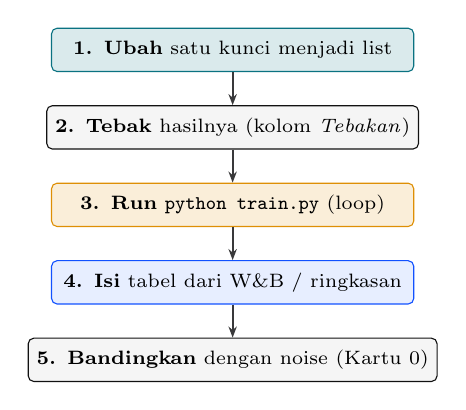
\begin{tikzpicture}[node distance=0.42cm]
            \node[lyrT, minimum width=4.6cm] (u) {\textbf{1. Ubah} satu kunci menjadi list};
            \node[lyr, minimum width=4.6cm, below=of u] (t) {\textbf{2. Tebak} hasilnya (kolom \emph{Tebakan})};
            \node[lyrO, minimum width=4.6cm, below=of t] (r) {\textbf{3. Run} \texttt{python train.py} (loop)};
            \node[lyrB, minimum width=4.6cm, below=of r] (i) {\textbf{4. Isi} tabel dari W\&B / ringkasan};
            \node[lyr, minimum width=4.6cm, below=of i] (b) {\textbf{5. Bandingkan} dengan noise (Kartu 0)};
            \draw[arr] (u) -- (t); \draw[arr] (t) -- (r); \draw[arr] (r) -- (i); \draw[arr] (i) -- (b);
        \end{tikzpicture}
        \end{center}
        {\scriptsize\color{dlMute} Kembalikan list ke satu nilai (baseline) sebelum pindah kartu.}
    \end{columns}
\end{frame}

%------------------------------------------------
\begin{frame}
    \frametitle{Parameter vs Hyperparameter}
    \framesubtitle{Siapa yang menentukan nilainya?}
    \footnotesize

    \vspace{4pt}
    \begin{center}
    \renewcommand{\arraystretch}{1.25}
    \begin{tabular}{p{2.6cm}p{5.0cm}p{5.0cm}}
        \toprule
        & \textbf{Parameter} $\bm{\theta}$ & \textbf{Hyperparameter} \\
        \midrule
        Contoh & bobot kernel konvolusi, bias, $\gamma/\beta$ BatchNorm, bobot attention & learning rate, optimizer, batch size, epoch, dropout, augmentasi, scheduler \\
        Ditentukan oleh & \textbf{gradient descent} (otomatis) & \textbf{Anda} (sebelum training) \\
        Jumlah & jutaan (ResNet-18: 11,2 M) & belasan (\texttt{CONFIG} di \texttt{train.py}) \\
        Dipilih memakai & data \textbf{train} & data \textbf{val} \\
        \bottomrule
    \end{tabular}
    \end{center}

    \vspace{0.2cm}
    \[
        \underbrace{\bm{\theta}^{*}(\bm{\lambda}) = \arg\min_{\bm{\theta}} \mathcal{L}_{\text{train}}(\bm{\theta};\bm{\lambda})}_{\text{training (loop dalam)}}
        \qquad
        \underbrace{\bm{\lambda}^{*} = \arg\max_{\bm{\lambda}} \text{Skor}_{\text{val}}\big(\bm{\theta}^{*}(\bm{\lambda})\big)}_{\text{hyperparameter tuning (loop luar)}}
    \]
    {\scriptsize\color{dlMute} $\bm{\lambda}$ = vektor hyperparameter. Setiap evaluasi loop luar = satu training penuh $\Rightarrow$ mahal, jadi harus dirancang dengan cermat.}
\end{frame}

%================================================
\section{Metodologi Eksperimen}
\bagian{BAGIAN 01 · METODOLOGI}{Eksperimen yang Jujur}{Split Data, Satu Kunci per Eksperimen, dan Prioritas}

%------------------------------------------------
\begin{frame}
    \frametitle{Dua Split, Dua Peran}
    \framesubtitle{Train untuk belajar, val untuk memilih}
    \footnotesize

    \begin{center}
    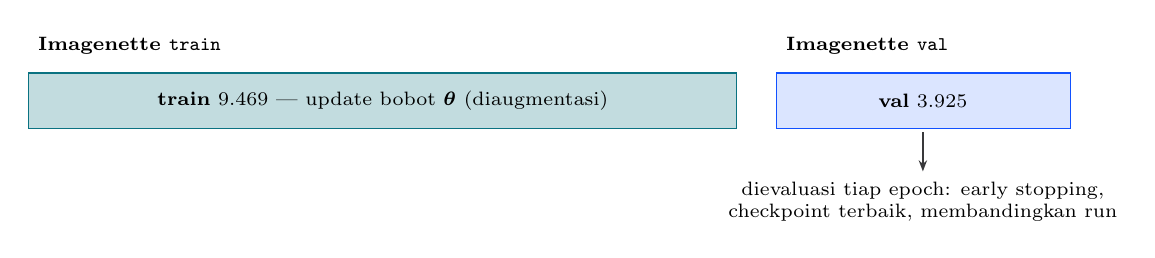
\begin{tikzpicture}[x=0.95cm]
        % Imagenette train -> train
        \node[font=\scriptsize\bfseries, anchor=west] at (0,1.05) {Imagenette \texttt{train}};
        \fill[dlTeal!25, draw=dlTeal] (0,0) rectangle (9.47,0.7);
        \node[font=\scriptsize] at (4.74,0.35) {\textbf{train} 9.469 --- update bobot $\bm{\theta}$ (diaugmentasi)};
        % Imagenette val -> val
        \node[font=\scriptsize\bfseries, anchor=west] at (10.0,1.05) {Imagenette \texttt{val}};
        \fill[dlBlue!15, draw=dlBlue] (10.0,0) rectangle (13.93,0.7);
        \node[font=\scriptsize] at (11.96,0.35) {\textbf{val} 3.925};
        % roles
        \draw[arr] (11.96,-0.05) -- (11.96,-0.55) node[below, font=\scriptsize, align=center] {dievaluasi tiap epoch: early stopping,\\checkpoint terbaik, membandingkan run};
    \end{tikzpicture}
    \end{center}

    \vspace{0.1cm}
    \begin{columns}[T]
        \column{0.48\textwidth}
        \begin{block}{Skor val sedikit optimistis}
            Kita \textbf{memilih} konfigurasi terbaik memakai val, jadi val ikut ``dilatih'' oleh keputusan kita. Untuk angka akhir yang jujur dibutuhkan data yang \con{tidak pernah} dipakai memilih.
        \end{block}
        \column{0.48\textwidth}
        \begin{exampleblock}{Analogi di Studio 2}
            Split lokal (\texttt{my\_val/}) = val Anda; tuning hanya pada \texttt{my\_val/}. \textbf{Validation set tersembunyi} milik asisten berperan sebagai data ``tak tersentuh'' tadi.
        \end{exampleblock}
    \end{columns}
\end{frame}

%------------------------------------------------
\begin{frame}
    \frametitle{Siklus Eksperimen}
    \framesubtitle{Hipotesis $\to$ satu perubahan $\to$ bukti}
    \footnotesize

    \begin{columns}[T]
        \column{0.50\textwidth}
        \begin{center}
        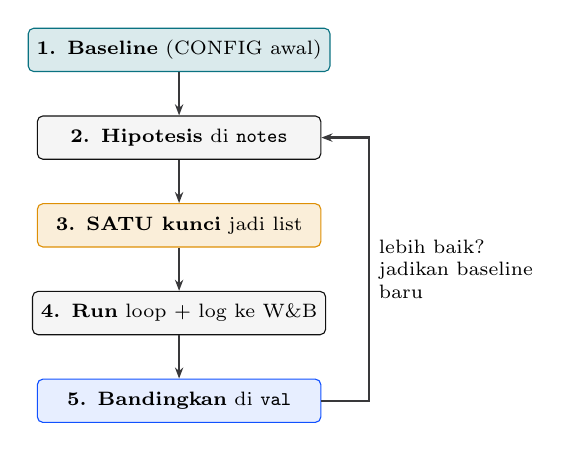
\begin{tikzpicture}[node distance=0.55cm]
            \node[lyrT, minimum width=3.6cm] (b) {\textbf{1. Baseline} (CONFIG awal)};
            \node[lyr, minimum width=3.6cm, below=of b] (h) {\textbf{2. Hipotesis} di \texttt{notes}};
            \node[lyrO, minimum width=3.6cm, below=of h] (c) {\textbf{3. SATU kunci} jadi list};
            \node[lyr, minimum width=3.6cm, below=of c] (r) {\textbf{4. Run} loop + log ke W\&B};
            \node[lyrB, minimum width=3.6cm, below=of r] (a) {\textbf{5. Bandingkan} di \texttt{val}};
            \draw[arr] (b) -- (h); \draw[arr] (h) -- (c); \draw[arr] (c) -- (r); \draw[arr] (r) -- (a);
            \draw[arr] (a.east) -- ++(0.6,0) |- node[pos=0.25, right, font=\scriptsize, align=left] {lebih baik?\\jadikan baseline\\baru} (h.east);
        \end{tikzpicture}
        \end{center}

        \column{0.46\textwidth}
        \textbf{Aturan main}
        \begin{itemize}
            \item \textbf{Satu kunci divariasikan per eksperimen} (boleh ditambah \texttt{model}) --- dua kunci sekaligus = efek tak bisa diatribusikan, dan jumlah run berlipat.
            \item \textbf{Seed tetap} (\texttt{seed=[42]}), split tetap.
            \item \textbf{Catat semuanya}, termasuk run yang gagal.
            \item \textbf{Ukur noise dulu}: ulangi baseline dengan \textbf{seed berbeda}; selisih lebih kecil dari noise = \con{bukan temuan}.
            \item Hipotesis ditulis \textbf{sebelum} run, bukan setelah melihat hasil.
        \end{itemize}
    \end{columns}
\end{frame}

%------------------------------------------------
\begin{frame}
    \frametitle{Kartu 0: Seberapa Besar Noise?}
    \framesubtitle{Baseline yang sama, seed berbeda}
    \footnotesize

    \begin{columns}[T]
        \column{0.40\textwidth}
        \begin{block}{List di CONFIG}
            {\ttfamily\scriptsize seed=[42, 1, 2]\\model=["resnet18", "vit\_tiny"]\\\# 3 x 2 = 6 run, $\pm$6 menit}
        \end{block}
        \textbf{Hipotesis} (tulis di \texttt{notes})
        \begin{itemize}
            \item Hasil \textbf{berbeda} walau konfigurasi sama: seed mengubah init head, urutan batch, dan augmentasi.
            \item Seed sama $\Rightarrow$ hasil identik: run ulang tanpa ganti seed \textbf{tidak} mengukur noise.
        \end{itemize}

        \column{0.56\textwidth}
        \vspace{2pt}
        \scriptsize
        \setlength{\tabcolsep}{4pt}
        \renewcommand{\arraystretch}{1.6}
        \arrayrulecolor{dlHairline}
        \begin{tabular}{|l|c|c|c|c|}
            \rowcolor{dlSoftCloud} & \multicolumn{2}{c|}{\textbf{ResNet-18}} & \multicolumn{2}{c|}{\textbf{ViT-Tiny}} \\
            \rowcolor{dlSoftCloud} \textbf{Seed} & \textbf{Best ep} & \textbf{Val acc} & \textbf{Best ep} & \textbf{Val acc} \\ \hline
            42 (baseline) & \hspace{0.75cm} & \hspace{0.75cm} & \hspace{0.75cm} & \hspace{0.75cm} \\ \hline
            1 & \hspace{0.75cm} & \hspace{0.75cm} & \hspace{0.75cm} & \hspace{0.75cm} \\ \hline
            2 & \hspace{0.75cm} & \hspace{0.75cm} & \hspace{0.75cm} & \hspace{0.75cm} \\ \hline
            \textbf{Rentang} (maks $-$ min) & \hspace{0.75cm} & \hspace{0.75cm} & \hspace{0.75cm} & \hspace{0.75cm} \\ \hline
        \end{tabular}
        \arrayrulecolor{black}

        \vspace{0.12cm}
        {\scriptsize Rentang ini = \textbf{ambang} untuk semua kartu berikutnya: selisih lebih kecil dari ini \con{belum tentu nyata}.}

        \vspace{0.1cm}
        {\scriptsize\color{dlMute} \textbf{Amati di W\&B:} group \texttt{seed}; \texttt{val/acc} keenam run bertumpuk di satu panel.}
    \end{columns}
\end{frame}

%------------------------------------------------
\begin{frame}
    \frametitle{Mana yang Dituning Lebih Dulu?}
    \framesubtitle{Prioritas untuk fine-tuning pretrained}
    \scriptsize

    \vspace{4pt}
    \begin{center}
    \renewcommand{\arraystretch}{1.18}
    \begin{tabular}{clp{4.4cm}p{3.9cm}}
        \toprule
        \textbf{Prio.} & \textbf{Hyperparameter} & \textbf{Kenapa} & \textbf{Kunci di \texttt{CONFIG}} \\
        \midrule
        \cellcolor{dlTeal!25}1 & Learning rate & paling sensitif; meleset satu orde = gagal & \texttt{lr}, \texttt{backbone\_lr\_mult} \\
        \cellcolor{dlTeal!25}1 & Pretrained \& strategi FT & menentukan titik awal optimasi & \texttt{finetune} \\
        \cellcolor{dlTeal!12}2 & Optimizer \& weight decay & berinteraksi kuat dengan lr & \texttt{optimizer}, \texttt{weight\_decay} \\
        \cellcolor{dlTeal!12}2 & Scheduler \& epoch & bentuk lr sepanjang training & \texttt{scheduler}, \texttt{warmup\_epochs} \\
        \cellcolor{dlTeal!12}2 & Batch size & noise gradien \& lr optimal & \texttt{batch\_size} \\
        \cellcolor{dlSoftCloud}3 & Regularisasi & penting saat data sedikit / overfit & \texttt{augment}, \texttt{dropout} \\
        \cellcolor{dlSoftCloud}3 & Early stopping & hemat waktu, checkpoint terbaik & \texttt{patience}, \texttt{monitor} \\
        \cellcolor{dlSoftCloud}4 & Arsitektur \& resolusi & ganti setelah resep training stabil & \texttt{model}, \texttt{img\_size} \\
        \bottomrule
    \end{tabular}
    \end{center}
    {\color{dlMute} Urutan mengikuti Google \textit{Deep Learning Tuning Playbook} dan Smith (2018): mulai dari efek terbesar, kunci nilainya, lalu lanjut.}
\end{frame}

%------------------------------------------------
\begin{frame}
    \frametitle{Diagnosis Dulu, Baru Tuning}
    \framesubtitle{loss train (garis) vs val (putus-putus)}
    \footnotesize

    \pgfmathsetmacro{\xbest}{2*ln(11.25)}
    \pgfmathsetmacro{\ybest}{0.9*exp(-\xbest/2)+0.04*\xbest+0.35}
    \begin{columns}[T]
        \column{0.32\textwidth}
        \centering\textbf{Underfitting}\\
        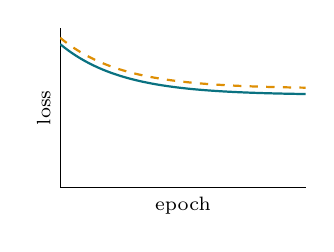
\begin{tikzpicture}
        \begin{axis}[dlaxis, width=4.7cm, height=3.6cm, xmin=0, xmax=12, ymin=0, ymax=2.5, xtick=\empty, ytick=\empty, xlabel={epoch}, ylabel={loss}]
            \addplot[dlTeal, domain=0:12, samples=60] {1.45+0.8*exp(-x/3)};
            \addplot[dlOrange, dashed, domain=0:12, samples=60] {1.55+0.8*exp(-x/3)};
        \end{axis}
        \end{tikzpicture}
        \begin{itemize}
            \item keduanya tinggi \& datar
            \item $\uparrow$ lr / epoch, pretrained, \con{kurangi} regularisasi, model lebih besar
        \end{itemize}

        \column{0.32\textwidth}
        \centering\textbf{Pas}\\
        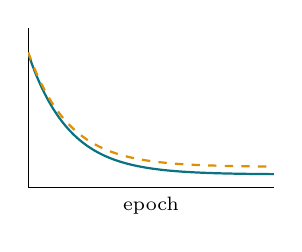
\begin{tikzpicture}
        \begin{axis}[dlaxis, width=4.7cm, height=3.6cm, xmin=0, xmax=12, ymin=0, ymax=2.5, xtick=\empty, ytick=\empty, xlabel={epoch}]
            \addplot[dlTeal, domain=0:12, samples=60] {0.2+1.9*exp(-x/2)};
            \addplot[dlOrange, dashed, domain=0:12, samples=60] {0.32+1.8*exp(-x/2)};
        \end{axis}
        \end{tikzpicture}
        \begin{itemize}
            \item turun bersama, gap kecil
            \item pertahankan; coba resolusi / model lain
        \end{itemize}

        \column{0.32\textwidth}
        \centering\textbf{Overfitting}\\
        \begin{tikzpicture}
        \begin{axis}[dlaxis, width=4.7cm, height=3.6cm, xmin=0, xmax=12, ymin=0, ymax=2.5, xtick=\empty, ytick=\empty, xlabel={epoch}]
            \addplot[dlTeal, domain=0:12, samples=60] {0.03+2.0*exp(-x/1.5)};
            \addplot[dlOrange, dashed, domain=0:12, samples=60] {0.9*exp(-x/2)+0.04*x+0.35};
            \draw[dlCharcoal, densely dotted] (axis cs:\xbest,0) -- (axis cs:\xbest,\ybest);
            \fill[dlCharcoal] (axis cs:\xbest,\ybest) circle (1.6pt);
            \node[font=\scriptsize, anchor=south] at (axis cs:\xbest,\ybest+0.25) {terbaik};
        \end{axis}
        \end{tikzpicture}
        \begin{itemize}
            \item train terus turun, val naik
            \item augmentasi, dropout, wd, label smoothing, MixUp, \textbf{early stopping}
        \end{itemize}
    \end{columns}
\end{frame}

%================================================
\section{Setup: Kode Eksperimen \& Weights \& Biases}
\bagian{BAGIAN 02 · SETUP}{Kode Eksperimen \& W\&B}{Tiga File, CONFIG Berisi List, Semua Run Tercatat}

%------------------------------------------------
\begin{frame}
    \frametitle{Dataset \& Lima Backbone}
    \framesubtitle{Imagenette 160 px · timm pretrained}
    \footnotesize

    \begin{columns}[T]
        \column{0.30\textwidth}
        \textbf{Imagenette} (J. Howard, fast.ai)
        \begin{itemize}
            \item subset \textbf{10 kelas} ImageNet yang mudah dibedakan (ikan tench, gereja, parasut, truk sampah, \ldots)
            \item 9.469 train · 3.925 val · versi 160 px $\approx$ 94 MB
            \item unduh otomatis lewat \texttt{torchvision}
        \end{itemize}
        {\scriptsize\color{dlMute} Kenapa bukan data sampah? Agar konfigurasi terbaik untuk kompetisi tetap menjadi temuan kelompok Anda sendiri.}

        \column{0.66\textwidth}
        \vspace{4pt}
        \scriptsize
        \setlength{\tabcolsep}{4pt}
        \renewcommand{\arraystretch}{1.2}
        \begin{tabular}{llrrr}
            \toprule
            \texttt{model} & \textbf{Keluarga} & \textbf{Param} & \textbf{s/epoch}$^{*}$ & \textbf{10 ep}$^{*}$ \\
            \midrule
            \texttt{resnet18} & CNN residual & 11,2 M & 4 & $\pm$0,8 menit \\
            \texttt{mobilenetv3} & depthwise + SE & 1,5 M & 5 & $\pm$0,9 menit \\
            \texttt{efficientnet\_b0} & compound scaling & 4,0 M & 7 & $\pm$1,3 menit \\
            \texttt{convnext\_atto} & CNN modern & 3,4 M & 5 & $\pm$1,0 menit \\
            \texttt{vit\_tiny} & Transformer & 5,5 M & 5 & $\pm$0,9 menit \\
            \bottomrule
        \end{tabular}

        \vspace{0.15cm}
        {\scriptsize $^{*}$terukur di RTX 5070 (batch 64, 160 px, AMP, 8 worker), termasuk validasi 3.925 citra; epoch pertama $\pm$5 s lebih lambat. Bottleneck-nya \textbf{loading data di CPU}, bukan ukuran model: MobileNetV3 (1,5 M) tidak lebih cepat dari ResNet-18 (11,2 M). Semua: varian \textbf{teringan} di keluarganya, satu file per arsitektur di \texttt{architectures/}, head 10 kelas via \texttt{timm.create\_model(..., num\_classes=10)}.}
    \end{columns}
\end{frame}

%------------------------------------------------
\begin{frame}
    \frametitle{Anatomi Kode}
    \framesubtitle{materials/hyperparameter-tuning/}
    \footnotesize

    \begin{columns}[T]
        \column{0.36\textwidth}
        {\ttfamily\scriptsize
        hyperparameter-tuning/\\
        +-- \textbf{train.py}\\
        |\hspace{2.2em}{\rmfamily\color{dlMute} CONFIG, loop, training, W\&B}\\
        +-- \textbf{datareader.py}\\
        |\hspace{2.2em}{\rmfamily\color{dlMute} Imagenette $\to$ DataLoader}\\
        +-- \textbf{models.py}\\
        |\hspace{2.2em}{\rmfamily\color{dlMute} pilih arsitektur + strategi FT}\\
        +-- \textbf{architectures/}\\
        \hspace*{2.4em}+-- resnet18.py\\
        \hspace*{2.4em}+-- mobilenetv3.py\\
        \hspace*{2.4em}+-- efficientnet\_b0.py\\
        \hspace*{2.4em}+-- convnext\_atto.py\\
        \hspace*{2.4em}+-- vit\_tiny.py\par}
        \vspace{0.1cm}
        {\scriptsize\color{dlMute} Tiap arsitektur: satu file berisi \texttt{build(...)}. Tanpa argparse: edit \texttt{CONFIG}, simpan, run. Run divergen ditandai \texttt{diverged}, loop lanjut.}

        \column{0.60\textwidth}
        \begin{center}
        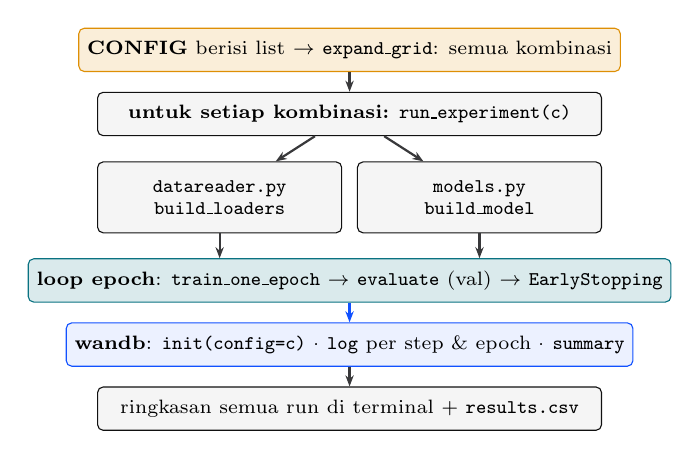
\begin{tikzpicture}[node distance=0.25cm]
            \node[lyrO, minimum width=6.4cm] (cfg) {\textbf{CONFIG} berisi list $\to$ \texttt{expand\_grid}: semua kombinasi};
            \node[lyr, below=of cfg, minimum width=6.4cm, fill=dlSoftCloud] (run) {\textbf{untuk setiap kombinasi:} \texttt{run\_experiment(c)}};
            \node[lyr, below=0.32cm of run, xshift=-1.65cm, minimum width=3.1cm, minimum height=0.9cm] (data) {\texttt{datareader.py}\\\texttt{build\_loaders}};
            \node[lyr, below=0.32cm of run, xshift=1.65cm, minimum width=3.1cm, minimum height=0.9cm] (model) {\texttt{models.py}\\\texttt{build\_model}};
            \node[lyrT, below=1.55cm of run, minimum width=6.4cm] (loop) {\textbf{loop epoch}: \texttt{train\_one\_epoch} $\to$ \texttt{evaluate} (val) $\to$ \texttt{EarlyStopping}};
            \node[lyrT, below=of loop, minimum width=6.4cm, fill=dlBlue!8, draw=dlBlue] (wb) {\textbf{wandb}: \texttt{init(config=c)} · \texttt{log} per step \& epoch · \texttt{summary}};
            \node[lyr, below=of wb, minimum width=6.4cm] (sum) {ringkasan semua run di terminal + \texttt{results.csv}};
            \draw[arr] (cfg) -- (run); \draw[arr] (run) -- (data); \draw[arr] (run) -- (model);
            \draw[arr] (data) -- (data |- loop.north); \draw[arr] (model) -- (model |- loop.north);
            \draw[arr, dlBlue] (loop) -- (wb); \draw[arr] (wb) -- (sum);
        \end{tikzpicture}
        \end{center}
    \end{columns}
\end{frame}

%------------------------------------------------
\begin{frame}[fragile]
    \frametitle{Blok CONFIG}
    \framesubtitle{List = dicoba satu per satu}
    \footnotesize

    \begin{columns}[T]
        \column{0.50\textwidth}
\begin{lstlisting}[style=py]
CONFIG = dict(
    # --- Data ---
    img_size=[160],         # 128 | 160 | 224
    train_fraction=[1.0],   # 0.1 = 10% data train
    augment=["basic"],      # none | basic | strong
    mixup_alpha=[0.0], cutmix_alpha=[0.0],
    # --- Model ---
    model=["resnet18", "vit_tiny"],
    finetune=["full_ft"],   # scratch | linear_probe
    backbone_lr_mult=[0.1], # lr backbone = lr * 0.1
    dropout=[0.0], drop_path=[0.0],
    # --- Optimizer ---
    optimizer=["adamw"],    # sgd | adam | adamw
                            # | nadam | rmsprop
    lr=[1e-3], weight_decay=[0.05],
    batch_size=[64], epochs=[10],
    label_smoothing=[0.0],
\end{lstlisting}
        \column{0.46\textwidth}
\begin{lstlisting}[style=py]
    # --- LR scheduler ---
    scheduler=["cosine"],   # none | step | cosine
                            # | onecycle | plateau
    warmup_epochs=[1],
    # --- Early stopping ---
    patience=[3],           # None = tanpa ES
    seed=[42],
    # --- Tetap (bukan list) ---
    monitor="val_loss",     # val_acc | val_f1
    wandb_project="if25-p6-hyperparameter",
    wandb_mode="online",    # offline | disabled
    notes="",               # tulis HIPOTESIS!
)
\end{lstlisting}
        \vspace{-0.1cm}
        {\scriptsize Jumlah run = \textbf{perkalian panjang semua list} (di atas: 2 run). Nama run \& group W\&B otomatis, mis.\ \texttt{vit\_tiny-optimizer=nadam}.}
    \end{columns}
\end{frame}

%------------------------------------------------
\begin{frame}[fragile]
    \frametitle{W\&B: Buku Catatan Eksperimen}
    \framesubtitle{Lima pemanggilan API}
    \footnotesize

    \begin{columns}[T]
        \column{0.53\textwidth}
\begin{lstlisting}[style=py]
# sekali per run, di dalam loop kombinasi
run = wandb.init(
    project="if25-p6-hyperparameter",
    name="vit_tiny-optimizer=nadam",
    group="optimizer",
    config=c,   # SEMUA hyperparameter run ini
    notes="nadam ~ adam?")
# per 10 step
wandb.log({"train/loss": loss, "train/lr": lr,
           "train/grad_norm": gnorm}, step=step)
# per epoch
wandb.log({"epoch": ep, "val/loss": vl,
           "val/acc": va, "val/f1": vf})
# akhir run: metrik di epoch terbaik
run.summary.update({"best/val_acc": acc})
wandb.log({"val/confusion_matrix":
           wandb.plot.confusion_matrix(...)})
wandb.finish()
\end{lstlisting}

        \column{0.43\textwidth}
        \textbf{Di dashboard, gunakan:}
        \begin{itemize}
            \item \textbf{Runs table}: urutkan menurut \texttt{best/val\_acc}, tampilkan kolom config.
            \item \textbf{Group / filter}: group \texttt{optimizer}, tag \texttt{vit\_tiny}.
            \item \textbf{Parallel coordinates}: hyperparameter mana yang berkorelasi dengan skor.
            \item \textbf{Line plot \texttt{train/lr}}: cek bentuk scheduler.
            \item \textbf{Report}: rangkuman untuk laporan Studio 2.
        \end{itemize}
        {\scriptsize\color{dlMute} Tanpa internet: \texttt{wandb\_mode="offline"}, lalu \texttt{wandb sync}.}
    \end{columns}
\end{frame}

%================================================
\section{Learning Rate, Optimizer \& Batch Size}
\bagian{BAGIAN 03 · OPTIMASI}{Learning Rate \& Optimizer}{Hyperparameter Paling Sensitif}

%------------------------------------------------
\begin{frame}
    \frametitle{Learning Rate: Ukuran Langkah}
    \framesubtitle{Hyperparameter paling sensitif}
    \footnotesize

    \begin{columns}[T]
        \column{0.52\textwidth}
        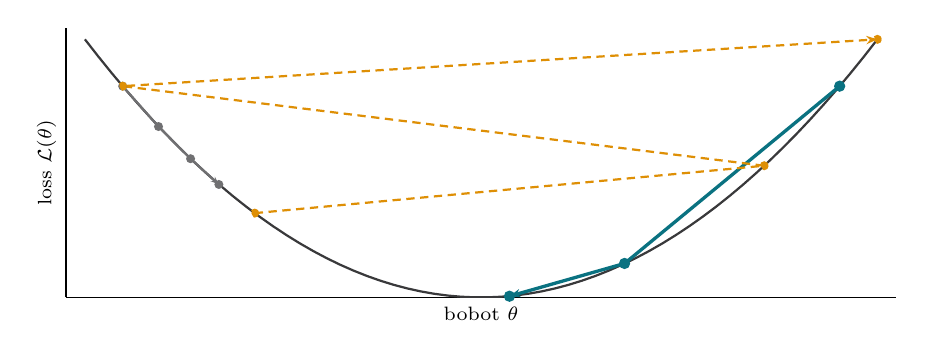
\begin{tikzpicture}
        \begin{axis}[dlaxis, width=\linewidth, height=5.0cm, xmin=-2.2, xmax=2.2, ymin=0, ymax=4.6,
            xtick=\empty, ytick=\empty, xlabel={bobot $\theta$}, ylabel={loss $\mathcal{L}(\theta)$}]
            \addplot[dlCharcoal, thick, domain=-2.1:2.1, samples=60] {x^2};
            % lr kecil: langkah pendek
            \addplot[dlMute, mark=*, mark size=1.2pt, -{Stealth[length=3pt]}] coordinates {(-1.9,3.61) (-1.71,2.92) (-1.54,2.37) (-1.39,1.93)};
            % lr pas
            \addplot[dlTeal, very thick, mark=*, mark size=1.4pt, -{Stealth[length=4pt]}] coordinates {(1.9,3.61) (0.76,0.58) (0.15,0.02)};
            % lr besar: melompat keluar
            \addplot[dlOrange, mark=*, mark size=1.2pt, densely dashed, -{Stealth[length=4pt]}] coordinates {(-1.2,1.44) (1.5,2.25) (-1.9,3.61) (2.1,4.41)};
        \end{axis}
        \end{tikzpicture}
        \[
            \theta_{t+1} = \theta_t - \eta\, \nabla_\theta \mathcal{L}(\theta_t)
        \]

        \column{0.44\textwidth}
        \begin{itemize}
            \item \textcolor{dlMute}{\textbf{$\eta$ kecil}}: tiap langkah aman tetapi pendek $\Rightarrow$ belum konvergen saat epoch habis (\textbf{underfit}).
            \item \pos{\textbf{$\eta$ pas}}: turun cepat lalu stabil.
            \item \con{\textbf{$\eta$ besar}}: melompati lembah, loss berosilasi atau \textbf{meledak} (NaN). \texttt{train.py} mendeteksinya dan menghentikan run (\texttt{diverged=True} di W\&B).
            \item lr optimal bergantung pada optimizer, batch size, dan backbone $\Rightarrow$ ganti salah satunya = cek lr ulang.
        \end{itemize}
        {\scriptsize\color{dlMute} Ilustrasi 1 dimensi; loss sebenarnya berdimensi jutaan.}
    \end{columns}
\end{frame}

%------------------------------------------------
\begin{frame}
    \frametitle{Kartu 1: Sweep Learning Rate}
    \framesubtitle{Skala log, bukan linear}
    \footnotesize

    \begin{columns}[T]
        \column{0.40\textwidth}
        \begin{block}{List di CONFIG}
            {\ttfamily\scriptsize lr=[1e-5, 1e-4, 1e-3, 1e-2, 1e-1]\\model=["resnet18", "vit\_tiny"]\\\# 5 x 2 = 10 run, $\pm$10 menit}
        \end{block}
        \textbf{Hipotesis} (tulis di \texttt{notes})
        \begin{itemize}
            \item Akurasi vs $\log_{10}\eta$ berbentuk \textbf{U terbalik}, untuk kedua arsitektur.
            \item lr terlalu besar: berhenti cepat (divergen / early stopping).
            \item lr terbaik ViT \textbf{belum tentu} sama dengan ResNet.
        \end{itemize}

        \column{0.56\textwidth}
        \vspace{2pt}
        \scriptsize
        \setlength{\tabcolsep}{4pt}
        \renewcommand{\arraystretch}{1.5}
        \arrayrulecolor{dlHairline}
        \begin{tabular}{|c|c|c|c|c|c|}
            \rowcolor{dlSoftCloud} & & \multicolumn{2}{c|}{\textbf{ResNet-18}} & \multicolumn{2}{c|}{\textbf{ViT-Tiny}} \\
            \rowcolor{dlSoftCloud} \textbf{\texttt{lr}} & \textbf{Tebakan} & \textbf{Henti ep} & \textbf{Val acc} & \textbf{Henti ep} & \textbf{Val acc} \\ \hline
            $10^{-5}$ & \hspace{0.75cm} & \hspace{0.75cm} & \hspace{0.75cm} & \hspace{0.75cm} & \hspace{0.75cm} \\ \hline
            $10^{-4}$ & \hspace{0.75cm} & \hspace{0.75cm} & \hspace{0.75cm} & \hspace{0.75cm} & \hspace{0.75cm} \\ \hline
            $10^{-3}$ & \hspace{0.75cm} & \hspace{0.75cm} & \hspace{0.75cm} & \hspace{0.75cm} & \hspace{0.75cm} \\ \hline
            $10^{-2}$ & \hspace{0.75cm} & \hspace{0.75cm} & \hspace{0.75cm} & \hspace{0.75cm} & \hspace{0.75cm} \\ \hline
            $10^{-1}$ & \hspace{0.75cm} & \hspace{0.75cm} & \hspace{0.75cm} & \hspace{0.75cm} & \hspace{0.75cm} \\ \hline
        \end{tabular}
        \arrayrulecolor{black}

        \vspace{0.12cm}
        {\scriptsize Setelah orde terbaik ketemu, haluskan dengan faktor $\pm3\times$: \texttt{lr=[3e-4, 1e-3, 3e-3]}.}

        \vspace{0.1cm}
        {\scriptsize\color{dlMute} \textbf{Amati di W\&B:} group \texttt{lr}; \texttt{train/loss} per step dan \texttt{val/acc}; panel \emph{Parallel coordinates} \texttt{lr} $\to$ \texttt{best/val\_acc}.}
    \end{columns}
\end{frame}

%------------------------------------------------
\begin{frame}
    \frametitle{SGD, Momentum, dan Adam}
    \framesubtitle{Aturan update yang dipilih \texttt{optimizer}}
    \footnotesize

    \begin{columns}[T]
        \column{0.48\textwidth}
        \textbf{SGD + momentum} (\texttt{"sgd"}, \texttt{momentum=0.9})
        \[
            \mathbf{v}_t = \mu\,\mathbf{v}_{t-1} + \mathbf{g}_t, \qquad
            \bm{\theta}_t = \bm{\theta}_{t-1} - \eta\,\mathbf{v}_t
        \]
        \begin{itemize}
            \item satu lr untuk semua bobot; momentum meredam zig-zag
            \item butuh lr lebih besar (umumnya $10^{-2}$) dan lebih sensitif terhadap lr
            \item sering sedikit lebih baik dalam generalisasi bila dituning cermat
        \end{itemize}

        \column{0.48\textwidth}
        \textbf{Adam} (\texttt{"adam"}): lr adaptif per bobot
        \[
            \mathbf{m}_t = \beta_1 \mathbf{m}_{t-1} + (1-\beta_1)\mathbf{g}_t, \quad
            \mathbf{s}_t = \beta_2 \mathbf{s}_{t-1} + (1-\beta_2)\mathbf{g}_t^{2}
        \]
        \[
            \bm{\theta}_t = \bm{\theta}_{t-1} - \eta\,\frac{\hat{\mathbf{m}}_t}{\sqrt{\hat{\mathbf{s}}_t}+\epsilon}
        \]
        \begin{itemize}
            \item bobot dengan gradien kecil mendapat langkah relatif besar
            \item lr default $10^{-3}$ biasanya ``langsung jalan''
            \item \texttt{"nadam"} (Dozat, 2016): Adam + momentum \textbf{Nesterov} --- $\hat{\mathbf{m}}_t$ ``melihat ke depan'' satu langkah
            \item \texttt{"rmsprop"}: hanya $\mathbf{s}_t$, tanpa $\mathbf{m}_t$ dan koreksi bias
        \end{itemize}
    \end{columns}
\end{frame}

%------------------------------------------------
\begin{frame}
    \frametitle{Kartu 2: Optimizer}
    \framesubtitle{Setiap optimizer punya lr idealnya}
    \footnotesize

    \begin{columns}[T]
        \column{0.42\textwidth}
        \begin{block}{List di CONFIG}
            {\ttfamily\scriptsize optimizer=["sgd", "adam", "adamw",\\\hspace*{5.6em}"nadam", "rmsprop"]\\model=["resnet18", "vit\_tiny"]\\\# 5 x 2 = 10 run, $\pm$10 menit}
        \end{block}
        \textbf{Hipotesis} (tulis di \texttt{notes})
        \begin{itemize}
            \item Pada lr $10^{-3}$, SGD tertinggal: butuh lr $\sim$10$\times$ lebih besar.
            \item NAdam $\approx$ Adam; AdamW unggul tipis (wd 0,05 decoupled).
        \end{itemize}
        {\scriptsize Lanjutan: \texttt{optimizer=["sgd"]}, \texttt{lr=[1e-3, 1e-2]}.}

        \column{0.54\textwidth}
        \vspace{2pt}
        \scriptsize
        \setlength{\tabcolsep}{4pt}
        \renewcommand{\arraystretch}{1.4}
        \arrayrulecolor{dlHairline}
        \begin{tabular}{|l|c|c|c|c|}
            \rowcolor{dlSoftCloud} & & & \multicolumn{2}{c|}{\textbf{Val acc}} \\
            \rowcolor{dlSoftCloud} \textbf{Optimizer} & \textbf{wd} & \textbf{Tebakan} & \textbf{ResNet-18} & \textbf{ViT-Tiny} \\ \hline
            SGD+mom. & 0,05 L2 & \hspace{0.75cm} & \hspace{0.75cm} & \hspace{0.75cm} \\ \hline
            Adam & 0,05 L2 & \hspace{0.75cm} & \hspace{0.75cm} & \hspace{0.75cm} \\ \hline
            AdamW & 0,05 dec. & \hspace{0.75cm} & \hspace{0.75cm} & \hspace{0.75cm} \\ \hline
            NAdam & 0,05 L2 & \hspace{0.75cm} & \hspace{0.75cm} & \hspace{0.75cm} \\ \hline
            RMSprop & 0,05 L2 & \hspace{0.75cm} & \hspace{0.75cm} & \hspace{0.75cm} \\ \hline
            SGD, lr $10^{-2}$ & 0,05 L2 & \hspace{0.75cm} & \hspace{0.75cm} & \hspace{0.75cm} \\ \hline
        \end{tabular}
        \arrayrulecolor{black}

        \vspace{0.12cm}
        {\scriptsize Semua lr $10^{-3}$ kecuali baris terakhir. L2 = decay lewat gradien; dec.\ = decoupled (AdamW). \texttt{momentum=0.9} untuk SGD \& RMSprop.}

        \vspace{0.1cm}
        {\scriptsize\color{dlMute} \textbf{Amati di W\&B:} group \texttt{optimizer}; kurva \texttt{val/acc} per optimizer di satu panel, pisahkan per tag \texttt{model}.}
    \end{columns}
\end{frame}

%------------------------------------------------
\begin{frame}
    \frametitle{Adam + L2 $\neq$ AdamW}
    \framesubtitle{Loshchilov \& Hutter (2019)}
    \footnotesize

    \begin{columns}[T]
        \column{0.55\textwidth}
        \textbf{Adam + L2} (\texttt{"adam"}, \texttt{weight\_decay}=$\lambda$): decay masuk ke gradien
        \[
            \mathbf{g}_t \leftarrow \nabla\mathcal{L} + \lambda\bm{\theta}
            \;\Rightarrow\;
            \bm{\theta} \leftarrow \bm{\theta} - \eta\,\frac{\hat{\mathbf{m}}_t}{\sqrt{\hat{\mathbf{s}}_t}+\epsilon}
        \]
        {\scriptsize $\lambda\bm{\theta}$ ikut \textbf{dinormalisasi} oleh $\sqrt{\hat{\mathbf{s}}_t}$: bobot dengan gradien kecil di-decay sangat kuat, yang gradiennya besar hampir tidak.}

        \vspace{0.15cm}
        \textbf{AdamW} (\texttt{"adamw"}): decay \textbf{dipisah} dari gradien
        \[
            \bm{\theta} \leftarrow \bm{\theta} - \eta\Big(\frac{\hat{\mathbf{m}}_t}{\sqrt{\hat{\mathbf{s}}_t}+\epsilon} + \lambda\bm{\theta}\Big)
        \]
        {\scriptsize Semua bobot menyusut dengan laju yang sama $\eta\lambda$ --- perilaku yang memang diinginkan dari weight decay.}

        \column{0.41\textwidth}
        \begin{block}{Kartu 2b: dua list sekaligus}
            {\ttfamily\scriptsize optimizer=["adam", "adamw"]\\weight\_decay=[0.0, 0.05]\\\# 2 x 2 x 2 model = 8 run}
            \begin{itemize}
                \item $\lambda=0$: Adam dan AdamW \textbf{identik}
                \item $\lambda=0{,}05$: Adam + L2 vs AdamW
            \end{itemize}
            Jika Adam + L2 paling rendah: $\lambda$ yang wajar untuk AdamW \con{terlalu kuat} sebagai L2.
        \end{block}
        {\scriptsize\color{dlMute} Di PyTorch: \texttt{torch.optim.Adam(weight\_decay=...)} = L2; \texttt{torch.optim.AdamW} = decoupled.}
    \end{columns}
\end{frame}

%------------------------------------------------
\begin{frame}
    \frametitle{Kartu 3: Batch Size}
    \framesubtitle{Goyal et al.\ (2017): linear scaling rule}
    \footnotesize

    \begin{columns}[T]
        \column{0.42\textwidth}
        \[
            B \to kB \quad\Rightarrow\quad \eta \to k\,\eta
        \]
        {\scriptsize Batch 4$\times$ lebih besar = langkah 4$\times$ lebih sedikit per epoch; kompensasi dengan lr 4$\times$ lebih besar (perlu warmup).}
        \begin{itemize}
            \item Batch besar: gradien lebih akurat, GPU efisien, tetapi \textbf{lebih sedikit update}.
            \item Batch kecil: gradien berisik (efek regularisasi), lebih lambat.
            \item \texttt{CUDA out of memory}: turunkan \texttt{batch\_size} \emph{dan} lr.
        \end{itemize}
        \textbf{Hipotesis}: 256 + $4\cdot10^{-3}$ menyamai baseline (64 + $10^{-3}$); 256 + $10^{-3}$ tertinggal.

        \column{0.54\textwidth}
        \begin{block}{List di CONFIG}
            {\ttfamily\scriptsize batch\_size=[32, 64, 256]\\lr=[1e-3, 4e-3]\\model=["resnet18"]   \# 3 x 2 = 6 run, $\pm$6 menit}
        \end{block}
        \vspace{2pt}
        \scriptsize
        \setlength{\tabcolsep}{4pt}
        \renewcommand{\arraystretch}{1.5}
        \arrayrulecolor{dlHairline}
        \begin{tabular}{|l|r|c|c|c|c|}
            \rowcolor{dlSoftCloud} & & & & \multicolumn{2}{c|}{\textbf{Val acc, lr}} \\
            \rowcolor{dlSoftCloud} \textbf{Batch} & \textbf{Step/ep} & \textbf{Tebakan} & \textbf{s/epoch} & \textbf{$10^{-3}$} & \textbf{$4\cdot10^{-3}$} \\ \hline
            32 & 295 & \hspace{0.6cm} & \hspace{0.6cm} & \hspace{0.6cm} & \hspace{0.6cm} \\ \hline
            64 (baseline) & 147 & \hspace{0.6cm} & \hspace{0.6cm} & \hspace{0.6cm} & \hspace{0.6cm} \\ \hline
            256 & 36 & \hspace{0.6cm} & \hspace{0.6cm} & \hspace{0.6cm} & \hspace{0.6cm} \\ \hline
        \end{tabular}
        \arrayrulecolor{black}

        \vspace{0.12cm}
        {\scriptsize Step/ep = $\lfloor 9.469 / B \rfloor$ (batch terakhir yang tidak penuh dibuang). Dua list = grid $3\times2$: kombinasi lain ikut dicoba sebagai bonus. Ada waktu? tambahkan \texttt{"vit\_tiny"}.}
    \end{columns}
\end{frame}

%================================================
\section{LR Scheduler \& Warmup}
\bagian{BAGIAN 04 · SCHEDULER}{LR Scheduler \& Warmup}{Learning Rate Tidak Harus Konstan}

%------------------------------------------------
\begin{frame}
    \frametitle{Bentuk-Bentuk Scheduler}
    \framesubtitle{lr relatif terhadap \texttt{lr} di CONFIG, 10 epoch}
    \footnotesize

    \begin{columns}[T]
        \column{0.58\textwidth}
        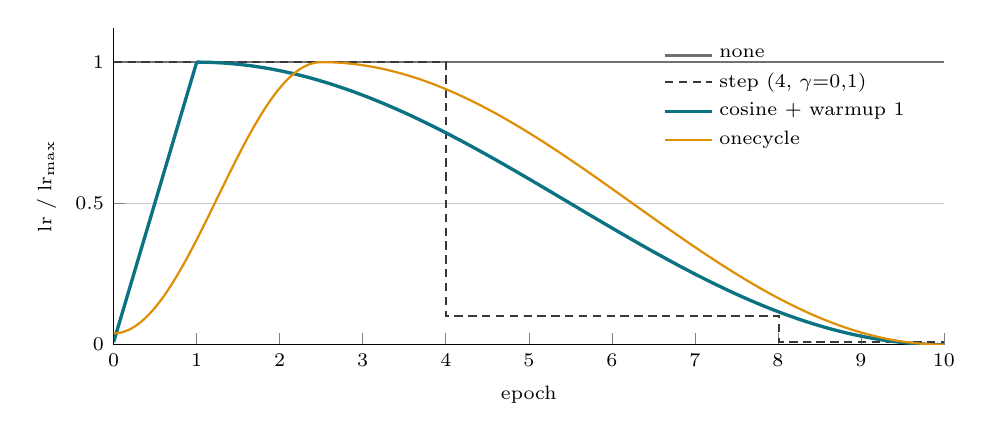
\begin{tikzpicture}
        \begin{axis}[dlaxis, width=\linewidth, height=5.6cm, xmin=0, xmax=10, ymin=0, ymax=1.12,
            xlabel={epoch}, ylabel={lr / lr$_{\max}$}, legend pos=north east, legend cell align=left]
            \addplot[dlMute, domain=0:10, samples=2] {1};
            \addlegendentry{none}
            \addplot[dlCharcoal, densely dashed, domain=0:10, samples=600, const plot] {0.1^(floor(x/4))};
            \addlegendentry{step (4, $\gamma$=0,1)}
            \addplot[dlTeal, very thick, domain=0:1, samples=20, forget plot] {0.01+0.99*x};
            \addplot[dlTeal, very thick, domain=1:10, samples=120] {0.5*(1+cos(180*(x-1)/9))};
            \addlegendentry{cosine + warmup 1}
            \addplot[dlOrange, domain=0:2.5, samples=60, forget plot] {0.04+0.96*(1-cos(180*x/2.5))/2};
            \addplot[dlOrange, domain=2.5:10, samples=120] {0.5*(1+cos(180*(x-2.5)/7.5))};
            \addlegendentry{onecycle}
        \end{axis}
        \end{tikzpicture}

        \column{0.38\textwidth}
        \begin{itemize}
            \item \textbf{step}: turun $\times\gamma$ tiap \texttt{step\_size} (= 4) epoch; sederhana, tapi waktu turunnya harus ditebak.
            \item \textbf{cosine}: turun mulus ke \texttt{min\_lr}; default modern (ConvNeXt, ViT).
            \item \textbf{onecycle}: naik lalu turun; lr puncak boleh lebih besar.
            \item \textbf{plateau}: turun $\times\gamma$ \textbf{hanya jika} \texttt{val\_loss} macet \texttt{plateau\_patience} epoch --- reaktif, tidak terjadwal.
        \end{itemize}
        {\scriptsize\color{dlMute} Di \texttt{train.py} semua di-\texttt{step()} per batch, kecuali plateau (per epoch).}
    \end{columns}
\end{frame}

%------------------------------------------------
\begin{frame}
    \frametitle{Kenapa Warmup?}
    \framesubtitle{Melindungi bobot pretrained di awal training}
    \footnotesize

    \begin{columns}[T]
        \column{0.50\textwidth}
        \begin{itemize}
            \item Di awal, \textbf{head baru diinisialisasi acak} $\Rightarrow$ loss besar, gradien besar dan ``berisik''.
            \item Gradien itu mengalir ke backbone; dengan lr penuh, fitur pretrained yang bagus bisa \con{rusak} di beberapa ratus langkah pertama.
            \item Adam: estimasi $\hat{\mathbf{s}}_t$ belum stabil pada langkah awal.
            \item \textbf{Warmup linear}: lr naik dari 1\% ke 100\% selama \texttt{warmup\_epochs}.
        \end{itemize}
        \[
            \eta_t = \eta_{\max}\Big(0{,}01 + 0{,}99\,\tfrac{t}{T_{\text{warm}}}\Big), \quad t < T_{\text{warm}}
        \]

        \column{0.46\textwidth}
        \begin{exampleblock}{Kombinasi yang dipakai di \texttt{train.py}}
            \texttt{LinearLR} (warmup) $\to$ \texttt{CosineAnnealingLR} via \texttt{SequentialLR}, di-step setiap batch.
        \end{exampleblock}
        \begin{itemize}
            \item ViT umumnya \textbf{lebih membutuhkan} warmup daripada CNN dengan BatchNorm.
            \item \texttt{backbone\_lr\_mult=0.1} adalah perlindungan kedua: backbone bergerak 10$\times$ lebih pelan dari head.
        \end{itemize}
    \end{columns}
\end{frame}

%------------------------------------------------
\begin{frame}
    \frametitle{Kartu 4: Scheduler}
    \framesubtitle{Efeknya bergantung pada lr}
    \footnotesize

    \begin{columns}[T]
        \column{0.40\textwidth}
        \begin{block}{List di CONFIG}
            {\ttfamily\scriptsize scheduler=["none", "step", "cosine",\\\hspace*{5.6em}"onecycle", "plateau"]\\model=["resnet18", "vit\_tiny"]\\\# 5 x 2 = 10 run, $\pm$10 menit}
        \end{block}
        {\scriptsize\textbf{4b}, lr kebesaran: \texttt{lr=[1e-2]}, \texttt{scheduler=["none", "cosine"]}, \texttt{warmup\_epochs=[0, 1]} (8 run)}

        \textbf{Hipotesis} (tulis di \texttt{notes})
        \begin{itemize}
            \item Pada lr yang sudah pas, scheduler mengubah sedikit.
            \item Pada lr kebesaran, cosine + warmup \textbf{menyelamatkan} run, terutama ViT.
        \end{itemize}

        \column{0.56\textwidth}
        \vspace{2pt}
        \scriptsize
        \setlength{\tabcolsep}{4pt}
        \renewcommand{\arraystretch}{1.25}
        \arrayrulecolor{dlHairline}
        \begin{tabular}{|l|c|c|c|c|}
            \rowcolor{dlSoftCloud} & & & \multicolumn{2}{c|}{\textbf{Val acc}} \\
            \rowcolor{dlSoftCloud} \textbf{Scheduler} & \textbf{lr} & \textbf{Tebakan} & \textbf{ResNet-18} & \textbf{ViT-Tiny} \\ \hline
            none & $10^{-3}$ & \hspace{0.75cm} & \hspace{0.75cm} & \hspace{0.75cm} \\ \hline
            step (4, 0,1) & $10^{-3}$ & \hspace{0.75cm} & \hspace{0.75cm} & \hspace{0.75cm} \\ \hline
            cosine, warmup 1 & $10^{-3}$ & \hspace{0.75cm} & \hspace{0.75cm} & \hspace{0.75cm} \\ \hline
            onecycle & $10^{-3}$ & \hspace{0.75cm} & \hspace{0.75cm} & \hspace{0.75cm} \\ \hline
            plateau & $10^{-3}$ & \hspace{0.75cm} & \hspace{0.75cm} & \hspace{0.75cm} \\ \hline
            none, warmup 0 & $10^{-2}$ & \hspace{0.75cm} & \hspace{0.75cm} & \hspace{0.75cm} \\ \hline
            none, warmup 1 & $10^{-2}$ & \hspace{0.75cm} & \hspace{0.75cm} & \hspace{0.75cm} \\ \hline
            cosine, warmup 0 & $10^{-2}$ & \hspace{0.75cm} & \hspace{0.75cm} & \hspace{0.75cm} \\ \hline
            cosine, warmup 1 & $10^{-2}$ & \hspace{0.75cm} & \hspace{0.75cm} & \hspace{0.75cm} \\ \hline
        \end{tabular}
        \arrayrulecolor{black}

        \vspace{0.12cm}
        {\scriptsize Plateau hanya turun jika \texttt{val\_loss} macet 2 epoch: dalam 10 epoch bisa saja \textbf{tidak pernah} turun.}

        \vspace{0.1cm}
        {\scriptsize\color{dlMute} \textbf{Amati di W\&B:} \texttt{train/lr} per step (bentuk kurva) dan \texttt{val/loss}.}
    \end{columns}
\end{frame}

%================================================
\section{Regularisasi \& Early Stopping}
\bagian{BAGIAN 05 · REGULARISASI}{Regularisasi \& Early Stopping}{Menutup Gap antara Train dan Val}

%------------------------------------------------
\begin{frame}
    \frametitle{Kartu 5: Memancing Overfitting}
    \framesubtitle{10\% data ($\approx$800 citra), tanpa regularisasi}
    \footnotesize

    \begin{columns}[T]
        \column{0.40\textwidth}
        \begin{block}{List di CONFIG}
            {\ttfamily\scriptsize train\_fraction=[0.1]\\augment=["none"]\\weight\_decay=[0.0]\\patience=[None]  \# tanpa ES\\epochs=[30]\\model=["resnet18", "vit\_tiny"]}
        \end{block}
        \textbf{Hipotesis} (tulis di \texttt{notes})
        \begin{itemize}
            \item Akurasi train mendekati 100\%, val tertinggal jauh: \textbf{gap} besar.
            \item Loss train terus turun; loss val mendatar atau naik.
        \end{itemize}

        \column{0.56\textwidth}
        \vspace{2pt}
        \scriptsize
        \setlength{\tabcolsep}{4pt}
        \renewcommand{\arraystretch}{1.6}
        \arrayrulecolor{dlHairline}
        \begin{tabular}{|c|c|c|c|c|}
            \rowcolor{dlSoftCloud} & \multicolumn{2}{c|}{\textbf{ResNet-18}} & \multicolumn{2}{c|}{\textbf{ViT-Tiny}} \\
            \rowcolor{dlSoftCloud} \textbf{Epoch} & \textbf{Train acc} & \textbf{Val acc} & \textbf{Train acc} & \textbf{Val acc} \\ \hline
            5 & \hspace{0.75cm} & \hspace{0.75cm} & \hspace{0.75cm} & \hspace{0.75cm} \\ \hline
            10 & \hspace{0.75cm} & \hspace{0.75cm} & \hspace{0.75cm} & \hspace{0.75cm} \\ \hline
            20 & \hspace{0.75cm} & \hspace{0.75cm} & \hspace{0.75cm} & \hspace{0.75cm} \\ \hline
            30 & \hspace{0.75cm} & \hspace{0.75cm} & \hspace{0.75cm} & \hspace{0.75cm} \\ \hline
        \end{tabular}
        \arrayrulecolor{black}

        \vspace{0.12cm}
        {\scriptsize Data train $\pm$950 citra: run cepat dan menjadi \textbf{baseline Kartu 6}. Studio 2 ($\pm$3.700 citra) juga termasuk ``data sedikit''.}

        \vspace{0.1cm}
        {\scriptsize\color{dlMute} \textbf{Amati di W\&B:} \texttt{epoch/train\_acc} vs \texttt{val/acc} dan \texttt{epoch/gap\_acc}.}
    \end{columns}
\end{frame}

%------------------------------------------------
\begin{frame}
    \frametitle{Dropout \& Stochastic Depth}
    \framesubtitle{\texttt{dropout} dan \texttt{drop\_path}}
    \footnotesize

    \begin{columns}[T]
        \column{0.48\textwidth}
        \textbf{Dropout} (Srivastava et al., 2014): matikan neuron acak
        \[
            \tilde{\mathbf{h}} = \frac{\mathbf{m}\odot\mathbf{h}}{1-p}, \qquad m_i \sim \text{Bernoulli}(1-p)
        \]
        \begin{center}
        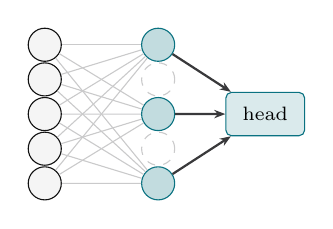
\begin{tikzpicture}[scale=0.8]
            \foreach \i in {0,...,4} { \node[circle, draw=dlInk, fill=dlSoftCloud, minimum size=0.42cm] (a\i) at (0,-\i*0.55) {}; }
            \foreach \i/\d in {0/0,1/1,2/0,3/1,4/0} {
                \ifnum\d=1 \node[circle, draw=dlHairline, dashed, minimum size=0.42cm] (b\i) at (1.8,-\i*0.55) {};
                \else \node[circle, draw=dlTeal, fill=dlTeal!25, minimum size=0.42cm] (b\i) at (1.8,-\i*0.55) {}; \fi }
            \foreach \i in {0,2,4} { \foreach \j in {0,...,4} { \draw[dlHairline] (a\j) -- (b\i); } }
            \node[lyrT, minimum width=1.0cm] (hd) at (3.5,-1.1) {head};
            \foreach \i in {0,2,4} { \draw[arr] (b\i) -- (hd); }
        \end{tikzpicture}
        \end{center}
        {\scriptsize Di timm: diterapkan \textbf{sebelum classifier} (\texttt{drop\_rate}). Saat \texttt{eval()} dropout otomatis mati.}

        \column{0.48\textwidth}
        \textbf{Stochastic depth / drop path} (Huang et al., 2016): matikan \textbf{seluruh cabang residual}
        \[
            \mathbf{x}_{l+1} = \mathbf{x}_l + \frac{b_l}{1-p}\, F_l(\mathbf{x}_l), \quad b_l \sim \text{Bernoulli}(1-p)
        \]
        \begin{itemize}
            \item jaringan ``acak lebih dangkal'' tiap batch $\Rightarrow$ ensemble implisit
            \item standar di ConvNeXt \& ViT (\texttt{drop\_path} 0,1--0,2)
            \item didukung kelima model di \texttt{architectures/} (timm \texttt{drop\_path\_rate})
        \end{itemize}
    \end{columns}
\end{frame}

%------------------------------------------------
\begin{frame}
    \frametitle{Weight Decay \& Label Smoothing}
    \framesubtitle{\texttt{weight\_decay} dan \texttt{label\_smoothing}}
    \footnotesize

    \begin{columns}[T]
        \column{0.48\textwidth}
        \textbf{Weight decay}: menarik bobot ke nol
        \[
            \mathcal{L}_{\text{total}} = \mathcal{L} + \frac{\lambda}{2}\lVert\bm{\theta}\rVert^2
            \;\Rightarrow\;
            \bm{\theta} \leftarrow (1-\eta\lambda)\,\bm{\theta} - \eta\,\mathbf{g}
        \]
        \begin{itemize}
            \item setara untuk SGD; \con{tidak setara} untuk Adam (lihat bagian optimizer)
            \item AdamW: $\lambda$ wajar 0,01--0,1; SGD: $10^{-4}$--$5\cdot10^{-4}$
        \end{itemize}

        \column{0.48\textwidth}
        \textbf{Label smoothing} (Szegedy et al., 2016): target tidak lagi 100\% yakin
        \[
            y_k^{\text{LS}} = (1-\varepsilon)\,y_k + \frac{\varepsilon}{K}
        \]
        \begin{center}
        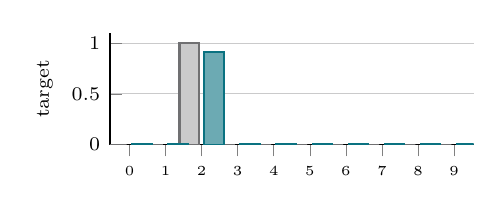
\begin{tikzpicture}
        \begin{axis}[dlaxis, ybar, bar width=7pt, width=6.2cm, height=3.0cm, ymin=0, ymax=1.1,
            xtick={0,...,9}, xticklabel style={font=\tiny}, ytick={0,0.5,1}, enlarge x limits=0.06, ylabel={target}]
            \addplot[fill=dlHairline, draw=dlMute] coordinates {(0,0)(1,0)(2,1)(3,0)(4,0)(5,0)(6,0)(7,0)(8,0)(9,0)};
            \addplot[fill=dlTeal!60, draw=dlTeal] coordinates {(0,0.01)(1,0.01)(2,0.91)(3,0.01)(4,0.01)(5,0.01)(6,0.01)(7,0.01)(8,0.01)(9,0.01)};
        \end{axis}
        \end{tikzpicture}
        \end{center}
        {\scriptsize abu-abu: one-hot · teal: $\varepsilon=0{,}1$, $K=10$. Mencegah logit membesar tanpa batas; model lebih terkalibrasi.}
    \end{columns}
\end{frame}

%------------------------------------------------
\begin{frame}
    \frametitle{Augmentasi Data, MixUp \& CutMix}
    \framesubtitle{\texttt{augment}, \texttt{mixup\_alpha}, \texttt{cutmix\_alpha}}
    \footnotesize

    \begin{columns}[T]
        \column{0.46\textwidth}
        \vspace{4pt}
        \renewcommand{\arraystretch}{1.2}
        \begin{tabular}{lp{4.4cm}}
            \toprule
            \texttt{augment} & Transformasi train \\
            \midrule
            \texttt{none} & resize + center crop (sama dengan val) \\
            \texttt{basic} & \texttt{RandomResizedCrop}(0,35--1) + flip horizontal \\
            \texttt{strong} & \texttt{basic} + \texttt{TrivialAugmentWide} + \texttt{RandomErasing}(p=0,25) \\
            \bottomrule
        \end{tabular}

        \vspace{0.2cm}
        {\scriptsize Citra val \textbf{tidak pernah} diaugmentasi (\texttt{datareader.py}). Augmentasi harus masuk akal untuk domain: flip vertikal untuk foto sampah? Mungkin. Untuk angka ``6'' vs ``9''? \con{Tidak}.}

        \column{0.50\textwidth}
        \textbf{MixUp} (Zhang et al., 2018): campur dua citra \emph{dan} labelnya
        \[
            \tilde{\mathbf{x}} = \lambda\mathbf{x}_i + (1-\lambda)\mathbf{x}_j, \quad
            \tilde{\mathbf{y}} = \lambda\mathbf{y}_i + (1-\lambda)\mathbf{y}_j
        \]
        dengan $\lambda \sim \text{Beta}(\alpha,\alpha)$, $\alpha$ = \texttt{mixup\_alpha}.


        \textbf{CutMix} (Yun et al., 2019): tempel potongan citra $j$ ke citra $i$; $\lambda$ = proporsi luas yang tersisa.
        \begin{itemize}
            \item label menjadi \textbf{soft} $\Rightarrow$ \texttt{CrossEntropyLoss} menerima probabilitas
            \item diterapkan per batch lewat \texttt{collate\_fn} (\texttt{v2.MixUp}, \texttt{v2.CutMix})
            \item butuh \textbf{lebih banyak epoch} agar manfaatnya terlihat
        \end{itemize}
    \end{columns}
\end{frame}

%------------------------------------------------
\begin{frame}
    \frametitle{Kartu 6: Regularisasi}
    \framesubtitle{Di atas konfigurasi Kartu 5}
    \footnotesize

    \begin{columns}[T]
        \column{0.40\textwidth}
        \begin{block}{List di CONFIG (satu per satu)}
            {\ttfamily\scriptsize augment=["none", "basic", "strong"]\\\# kembalikan augment=["none"], lalu:\\dropout=[0.0, 0.5]\\weight\_decay=[0.0, 0.05]\\label\_smoothing=[0.0, 0.1]\\mixup\_alpha=[0.2], cutmix\_alpha=[1.0]}
        \end{block}
        \textbf{Hipotesis} (tulis di \texttt{notes})
        \begin{itemize}
            \item Augmentasi paling ampuh saat data sedikit.
            \item Gap mengecil $\neq$ val acc pasti naik.
        \end{itemize}

        \column{0.56\textwidth}
        \vspace{2pt}
        \scriptsize
        \setlength{\tabcolsep}{4pt}
        \renewcommand{\arraystretch}{1.3}
        \arrayrulecolor{dlHairline}
        \begin{tabular}{|l|c|c|c|c|c|}
            \rowcolor{dlSoftCloud} & & \multicolumn{2}{c|}{\textbf{ResNet-18}} & \multicolumn{2}{c|}{\textbf{ViT-Tiny}} \\
            \rowcolor{dlSoftCloud} \textbf{Perubahan} & \textbf{Tebakan} & \textbf{Gap$^{*}$} & \textbf{Val} & \textbf{Gap$^{*}$} & \textbf{Val} \\ \hline
            (Kartu 5) & \hspace{0.6cm} & \hspace{0.6cm} & \hspace{0.6cm} & \hspace{0.6cm} & \hspace{0.6cm} \\ \hline
            aug.\ basic & \hspace{0.6cm} & \hspace{0.6cm} & \hspace{0.6cm} & \hspace{0.6cm} & \hspace{0.6cm} \\ \hline
            aug.\ strong & \hspace{0.6cm} & \hspace{0.6cm} & \hspace{0.6cm} & \hspace{0.6cm} & \hspace{0.6cm} \\ \hline
            dropout 0,5 & \hspace{0.6cm} & \hspace{0.6cm} & \hspace{0.6cm} & \hspace{0.6cm} & \hspace{0.6cm} \\ \hline
            wd 0,05 & \hspace{0.6cm} & \hspace{0.6cm} & \hspace{0.6cm} & \hspace{0.6cm} & \hspace{0.6cm} \\ \hline
            label smooth.\ 0,1 & \hspace{0.6cm} & \hspace{0.6cm} & \hspace{0.6cm} & \hspace{0.6cm} & \hspace{0.6cm} \\ \hline
            MixUp + CutMix & \hspace{0.6cm} & \hspace{0.6cm} & \hspace{0.6cm} & \hspace{0.6cm} & \hspace{0.6cm} \\ \hline
        \end{tabular}
        \arrayrulecolor{black}

        \vspace{0.12cm}
        {\scriptsize $^{*}$train $-$ val di epoch terakhir; dengan augmentasi/MixUp akurasi train dihitung pada citra teraugmentasi, jadi gap bisa negatif. List berisi nilai Kartu 5 (mis.\ \texttt{0.0}) membuat baris baseline ikut dijalankan ulang. Noise di data sedikit lebih besar: \texttt{seed=[42, 1]}.}

        \vspace{0.1cm}
        {\scriptsize\color{dlMute} \textbf{Amati di W\&B:} \texttt{epoch/gap\_acc} semua run dalam satu panel.}
    \end{columns}
\end{frame}

%------------------------------------------------
\begin{frame}
    \frametitle{Kartu 7: Early Stopping}
    \framesubtitle{\texttt{patience}, \texttt{min\_delta}, \texttt{monitor}}
    \footnotesize

    \begin{columns}[T]
        \column{0.50\textwidth}
        \textbf{Aturan} (kelas \texttt{EarlyStopping} di \texttt{train.py}): berhenti jika
        \[
            \underbrace{m_t > m^{*} - \delta}_{\text{tidak membaik}} \quad \text{selama } P \text{ epoch berturut-turut}
        \]
        \begin{itemize}
            \item $m$ = \texttt{monitor} (\texttt{val\_loss} turun; \texttt{val\_acc}/\texttt{val\_f1} naik), $\delta$ = \texttt{min\_delta}, $P$ = \texttt{patience}
            \item setiap kali membaik: \textbf{simpan checkpoint}; hasil run = metrik di epoch terbaik, \emph{bukan} epoch terakhir
            \item Studio 2 dinilai dengan macro-F1 $\Rightarrow$ \texttt{monitor="val\_f1"}
        \end{itemize}

        \column{0.46\textwidth}
        \begin{block}{List di CONFIG}
            {\ttfamily\scriptsize patience=[None, 5, 2]   \# None = penuh\\epochs=[30]\\model=["resnet18"]   \# 3 run, $\pm$6 menit}
        \end{block}
        \vspace{2pt}
        \scriptsize
        \setlength{\tabcolsep}{4pt}
        \renewcommand{\arraystretch}{1.5}
        \arrayrulecolor{dlHairline}
        \begin{tabular}{|l|c|c|c|}
            \rowcolor{dlSoftCloud} \textbf{\texttt{patience}} & \textbf{None} & \textbf{5} & \textbf{2} \\ \hline
            Epoch dijalankan & \hspace{0.75cm} & \hspace{0.75cm} & \hspace{0.75cm} \\ \hline
            Epoch terbaik & \hspace{0.75cm} & \hspace{0.75cm} & \hspace{0.75cm} \\ \hline
            Waktu (menit) & \hspace{0.75cm} & \hspace{0.75cm} & \hspace{0.75cm} \\ \hline
            Val acc terbaik & \hspace{0.75cm} & \hspace{0.75cm} & \hspace{0.75cm} \\ \hline
        \end{tabular}
        \arrayrulecolor{black}

        \vspace{0.1cm}
        \textbf{Hipotesis}: val acc terbaik hampir sama, waktu jauh lebih singkat; $P$ terlalu kecil berhenti di plateau sementara.
    \end{columns}
\end{frame}

%================================================
\section{Strategi Fine-tuning \& Pilihan Model}
\bagian{BAGIAN 06 · FINE-TUNING}{Fine-tuning \& CNN vs ViT}{Bagian Mana yang Dilatih, dan Seberapa Cepat}

%------------------------------------------------
\begin{frame}
    \frametitle{Empat Strategi Melatih Backbone}
    \framesubtitle{Bagian mana yang belajar?}
    \scriptsize

    \begin{center}
    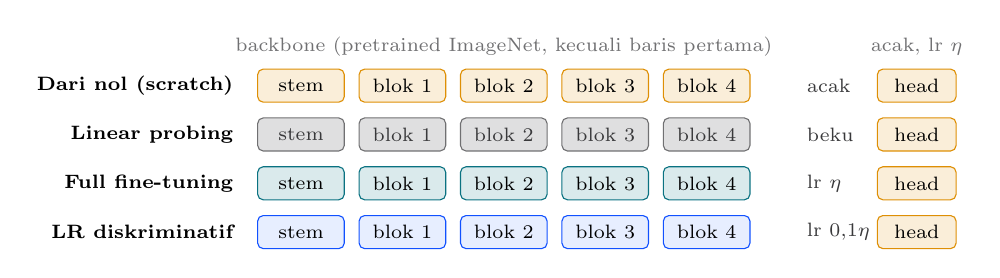
\begin{tikzpicture}[x=0.92cm, y=0.62cm]
        \foreach \row/\name/\s/\c in {0/Dari nol (scratch)/acak/lyrO, 1/Linear probing/beku/lyrG, 2/Full fine-tuning/lr $\eta$/lyrT, 3/LR diskriminatif/lr $0{,}1\eta$/lyrB} {
            \node[font=\scriptsize\bfseries, anchor=east] at (2.6,-\row) {\name};
            \foreach \b/\lab in {0/stem, 1/blok 1, 2/blok 2, 3/blok 3, 4/blok 4} {
                \node[\c, minimum width=1.1cm, minimum height=0.42cm] at (3.4+\b*1.4,-\row) {\lab};
            }
            \node[font=\scriptsize, anchor=west, text=dlCharcoal] at (10.25,-\row) {\s};
        }
        \foreach \row in {0,1,2,3} { \node[lyrO, minimum width=1.0cm, minimum height=0.42cm] at (11.9,-\row) {head}; }
        \node[font=\scriptsize, text=dlMute] at (11.9,0.8) {acak, lr $\eta$};
        \node[font=\scriptsize, text=dlMute] at (6.2,0.8) {backbone (pretrained ImageNet, kecuali baris pertama)};
    \end{tikzpicture}
    \end{center}

    \renewcommand{\arraystretch}{1.1}
    \begin{center}
    \begin{tabular}{llp{3.4cm}p{3.3cm}}
        \toprule
        \textbf{Strategi} & \textbf{CONFIG} & \textbf{Cocok ketika} & \textbf{Risiko} \\
        \midrule
        Scratch & \texttt{finetune="scratch"} & domain jauh + data banyak & lambat, haus data \\
        Linear probing & \texttt{finetune="linear\_probe"} & data sangat sedikit & fitur tak beradaptasi \\
        Full FT & \texttt{"full\_ft"}, \texttt{backbone\_lr\_mult=1.0} & data cukup & fitur rusak bila lr besar \\
        LR diskriminatif & \texttt{"full\_ft"}, \texttt{backbone\_lr\_mult=0.1} & default yang aman & +1 hyperparameter \\
        \bottomrule
    \end{tabular}
    \end{center}
\end{frame}

%------------------------------------------------
\begin{frame}
    \frametitle{Kartu 8: Strategi Fine-tuning}
    \framesubtitle{ResNet-18 \& ViT-Tiny, data penuh}
    \footnotesize

    \begin{columns}[T]
        \column{0.42\textwidth}
        \begin{block}{List di CONFIG}
            {\ttfamily\scriptsize finetune=["scratch", "linear\_probe",\\\hspace*{5.0em}"full\_ft"]\\model=["resnet18", "vit\_tiny"]\\\# 3 x 2 = 6 run, $\pm$6 menit}
        \end{block}
        {\scriptsize Lanjutan: \texttt{finetune=["full\_ft"]}, \texttt{backbone\_lr\_mult=[1.0, 0.1]} (4 run).}

        \textbf{Hipotesis} (tulis di \texttt{notes})
        \begin{itemize}
            \item Scratch tertinggal \textbf{jauh}: bobot pretrained adalah hyperparameter terpenting.
            \item Linear probe $\approx$ full FT di Imagenette, karena kelasnya \emph{adalah} kelas ImageNet.
        \end{itemize}

        \column{0.54\textwidth}
        \vspace{2pt}
        \scriptsize
        \setlength{\tabcolsep}{4pt}
        \renewcommand{\arraystretch}{1.5}
        \arrayrulecolor{dlHairline}
        \begin{tabular}{|l|c|c|c|c|}
            \rowcolor{dlSoftCloud} & & & \multicolumn{2}{c|}{\textbf{Val acc}} \\
            \rowcolor{dlSoftCloud} \textbf{Strategi} & \textbf{Dilatih (R18)} & \textbf{Tebakan} & \textbf{ResNet-18} & \textbf{ViT-Tiny} \\ \hline
            Scratch & 11,2 M & \hspace{0.75cm} & \hspace{0.75cm} & \hspace{0.75cm} \\ \hline
            Linear probe & 5 K & \hspace{0.75cm} & \hspace{0.75cm} & \hspace{0.75cm} \\ \hline
            Full FT $\times$1 & 11,2 M & \hspace{0.75cm} & \hspace{0.75cm} & \hspace{0.75cm} \\ \hline
            Full FT $\times$0,1 & 11,2 M & \hspace{0.75cm} & \hspace{0.75cm} & \hspace{0.75cm} \\ \hline
        \end{tabular}
        \arrayrulecolor{black}

        \vspace{0.12cm}
        {\scriptsize $\times$1 / $\times$0,1 = \texttt{backbone\_lr\_mult}. Data sampah berbeda domain dari ImageNet $\Rightarrow$ ulangi perbandingan ini di data Anda.}

        \vspace{0.1cm}
        {\scriptsize\color{dlMute} \textbf{Amati di W\&B:} \texttt{val/acc} epoch 1: pretrained langsung tinggi, scratch mulai dari $\approx$10\%.}
    \end{columns}
\end{frame}

%------------------------------------------------
\begin{frame}
    \frametitle{Kartu 9: CNN vs ViT}
    \framesubtitle{Resep sama, backbone berbeda}
    \footnotesize

    \begin{columns}[T]
        \column{0.42\textwidth}
        \begin{block}{List di CONFIG}
            {\ttfamily\scriptsize model=["resnet18", "mobilenetv3",\\\hspace*{3.2em}"efficientnet\_b0",\\\hspace*{3.2em}"convnext\_atto", "vit\_tiny"]\\train\_fraction=[1.0, 0.1]\\\# 5 x 2 = 10 run, $\pm$8 menit}
        \end{block}
        \textbf{Hipotesis} (tulis di \texttt{notes})
        \begin{itemize}
            \item ``ViT haus data'' berlaku untuk training \textbf{dari nol}. Dengan pretraining ImageNet-21k, apakah ViT tetap kalah di 10\% data?
            \item Ganti backbone = \textbf{cek lr ulang}: lr $10^{-3}$ belum tentu cocok untuk ViT.
        \end{itemize}

        \column{0.54\textwidth}
        \vspace{2pt}
        \scriptsize
        \setlength{\tabcolsep}{4pt}
        \renewcommand{\arraystretch}{1.55}
        \arrayrulecolor{dlHairline}
        \begin{tabular}{|l|r|c|c|c|}
            \rowcolor{dlSoftCloud} \textbf{Model} & \textbf{Param} & \textbf{Tebakan} & \textbf{Val 100\%} & \textbf{Val 10\%} \\ \hline
            ResNet-18 & 11,2 M & \hspace{0.75cm} & \hspace{0.75cm} & \hspace{0.75cm} \\ \hline
            MobileNetV3-S & 1,5 M & \hspace{0.75cm} & \hspace{0.75cm} & \hspace{0.75cm} \\ \hline
            EfficientNet-B0 & 4,0 M & \hspace{0.75cm} & \hspace{0.75cm} & \hspace{0.75cm} \\ \hline
            ConvNeXt-Atto & 3,4 M & \hspace{0.75cm} & \hspace{0.75cm} & \hspace{0.75cm} \\ \hline
            ViT-Tiny/16 & 5,5 M & \hspace{0.75cm} & \hspace{0.75cm} & \hspace{0.75cm} \\ \hline
        \end{tabular}
        \arrayrulecolor{black}

        \vspace{0.12cm}
        {\scriptsize CNN: lokalitas \& translation equivariance ``dibangun'' di konvolusi. ViT: attention global antar-patch $16\times16$; di 160 px = $10\times10$ patch (\texttt{img\_size=[160]}). Run 10\% data $<$1 menit.}

        \vspace{0.1cm}
        {\scriptsize\color{dlMute} \textbf{Amati di W\&B:} \texttt{best\_epoch}; jika terbaik di epoch 1--2, lr kemungkinan kebesaran.}
    \end{columns}
\end{frame}

%================================================
\section{Strategi Pencarian \& Resep Praktis}
\bagian{BAGIAN 07 · PENCARIAN}{Strategi Pencarian \& Resep}{Dari Tebakan Manual ke Pencarian Sistematis}

%------------------------------------------------
\begin{frame}
    \frametitle{Grid Search vs Random Search}
    \framesubtitle{Bergstra \& Bengio (2012)}
    \footnotesize

    \begin{columns}[T]
        \column{0.58\textwidth}
        \begin{center}
        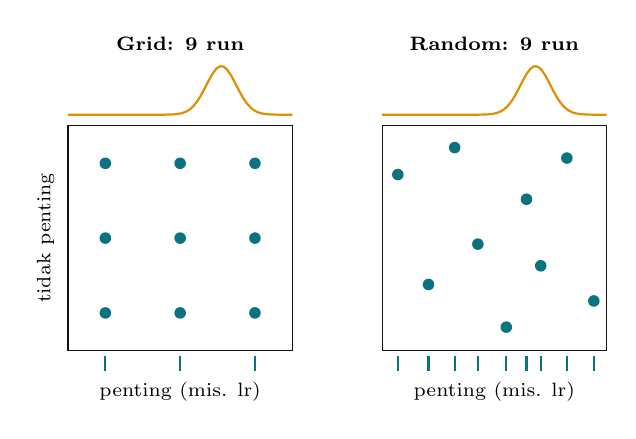
\begin{tikzpicture}[scale=0.95]
            % ---- Grid ----
            \begin{scope}
                \draw[dlInk] (0,0) rectangle (3,3);
                \foreach \x in {0.5,1.5,2.5} { \foreach \y in {0.5,1.5,2.5} { \fill[dlTeal] (\x,\y) circle (2.2pt); } }
                \draw[dlOrange, thick, domain=0:3, samples=60] plot (\x, {3.15+0.65*exp(-((\x-2.05)^2)/0.08)});
                \foreach \x in {0.5,1.5,2.5} { \draw[dlTeal, thick] (\x,-0.08) -- (\x,-0.28); }
                \node[font=\scriptsize] at (1.5,-0.55) {penting (mis. lr)};
                \node[font=\scriptsize, rotate=90] at (-0.3,1.5) {tidak penting};
                \node[font=\scriptsize\bfseries] at (1.5,4.1) {Grid: 9 run};
            \end{scope}
            % ---- Random ----
            \begin{scope}[xshift=4.2cm]
                \draw[dlInk] (0,0) rectangle (3,3);
                \foreach \x/\y in {0.21/2.35, 0.62/0.88, 0.97/2.71, 1.28/1.42, 1.66/0.31, 1.93/2.02, 2.12/1.13, 2.47/2.57, 2.83/0.66} {
                    \fill[dlTeal] (\x,\y) circle (2.2pt); \draw[dlTeal, thick] (\x,-0.08) -- (\x,-0.28); }
                \draw[dlOrange, thick, domain=0:3, samples=60] plot (\x, {3.15+0.65*exp(-((\x-2.05)^2)/0.08)});
                \node[font=\scriptsize] at (1.5,-0.55) {penting (mis. lr)};
                \node[font=\scriptsize\bfseries] at (1.5,4.1) {Random: 9 run};
            \end{scope}
        \end{tikzpicture}
        \end{center}

        \column{0.38\textwidth}
        \begin{itemize}
            \item Grid: 9 run, tetapi hanya \con{3 nilai berbeda} untuk hyperparameter yang penting.
            \item Random: 9 run $\Rightarrow$ \pos{9 nilai berbeda} untuk setiap dimensi.
            \item Kurva oranye = skor vs hyperparameter penting; puncaknya sempit dan mudah terlewat oleh grid.
            \item Sampling lr dalam \textbf{skala log}: $\eta = 10^{u}$, $u\sim\mathcal{U}(-5,-1)$.
            \item List di \texttt{CONFIG} kita = \textbf{grid search}: cocok untuk 1--2 kunci, mahal untuk banyak kunci.
        \end{itemize}
    \end{columns}
\end{frame}

%------------------------------------------------
\begin{frame}[fragile]
    \frametitle{Coarse-to-Fine \& W\&B Sweeps}
    \framesubtitle{Langkah berikutnya setelah tuning manual}
    \footnotesize

    \begin{columns}[T]
        \column{0.46\textwidth}
        \textbf{Coarse-to-fine}
        \begin{enumerate}
            \item \textbf{Kasar}: lr $\in\{10^{-5},\dots,10^{-1}\}$, epoch pendek, \texttt{train\_fraction=0.3}.
            \item \textbf{Sempit}: sekitar 2--3 nilai terbaik, data penuh.
            \item \textbf{Halus}: hyperparameter prioritas 2--3 pada lr terbaik.
            \item \textbf{Konfirmasi}: ulangi konfigurasi terbaik dengan 2--3 seed.
        \end{enumerate}
        {\scriptsize\color{dlMute} List di \texttt{CONFIG} di kelas = langkah 1--2 (mis.\ \texttt{seed=[42, 1, 2]} untuk langkah 4). W\&B Sweeps mengotomatiskan langkah 2--3.}

        \column{0.50\textwidth}
        \textbf{W\&B Sweeps} (Bayesian / random / grid)
\begin{lstlisting}[style=py]
sweep = {
  "method": "random",       # "bayes" | "grid"
  "metric": {"name": "best/val_acc",
             "goal": "maximize"},
  "parameters": {
    "lr": {"distribution": "log_uniform_values",
           "min": 1e-5, "max": 1e-2},
    "dropout": {"values": [0.0, 0.2, 0.5]},
    "optimizer": {"values": ["sgd", "adamw"]},
  },
}
sweep_id = wandb.sweep(sweep, project="if25-p6")
wandb.agent(sweep_id, function=..., count=20)
\end{lstlisting}
        {\scriptsize\color{dlMute} Agar bisa di-sweep, \texttt{run\_experiment} perlu membaca nilai dari \texttt{wandb.config} setelah \texttt{wandb.init()}, bukan dari \texttt{CONFIG}.}
    \end{columns}
\end{frame}

%------------------------------------------------
\begin{frame}
    \frametitle{Resep Praktis untuk Studio 2}
    \framesubtitle{Urutan kerja yang disarankan}
    \footnotesize

    \begin{columns}[T]
        \column{0.58\textwidth}
        \begin{enumerate}
            \item \textbf{Baseline} starter kit + split lokal tetap; ukur noise dengan 2--3 seed (Kartu 0).
            \item \textbf{Pretrained}; bandingkan \textbf{linear probe} vs \textbf{full FT} di data sendiri (Kartu 8).
            \item \textbf{Sweep lr} dalam skala log; ganti optimizer/batch/backbone $\Rightarrow$ cek lr ulang.
            \item \textbf{AdamW} (bukan Adam + L2), cosine + warmup 1 epoch, \texttt{backbone\_lr\_mult} 0,1.
            \item Lihat kurva: gap besar $\Rightarrow$ augmentasi dulu, lalu label smoothing / MixUp / dropout.
            \item \textbf{Early stopping} pada \texttt{val\_f1} (metrik kompetisi), patience 3--5 (lebih besar untuk OneCycle).
            \item Baru setelah itu: \textbf{backbone lain} \& resolusi lebih besar.
        \end{enumerate}

        \column{0.38\textwidth}
        \begin{block}{Jangan}
            \begin{itemize}
                \item mengubah 3 hal sekaligus
                \item memilih model memakai skor preview kompetisi
                \item mengklaim selisih $<$ noise
                \item lupa mencatat run yang gagal
            \end{itemize}
        \end{block}
        \begin{exampleblock}{Bawa pulang}
            Bandingkan tabel kartu Anda dengan tabel prioritas di awal: \textbf{mana yang benar-benar berefek} melebihi noise?
        \end{exampleblock}
    \end{columns}
\end{frame}

%------------------------------------------------
\begin{frame}
    \frametitle{Aktivitas Kelas}
    \framesubtitle{30 menit, per kelompok Studio 2}
    \footnotesize

    \begin{columns}[T]
        \column{0.55\textwidth}
        \begin{enumerate}
            \item Buat proyek W\&B kelompok; isi \texttt{wandb\_entity}.
            \item Jalankan \textbf{baseline} \texttt{train.py} apa adanya (catat \texttt{best/val\_acc}).
            \item Setiap anggota memilih \textbf{satu} hyperparameter dari tabel prioritas, menulis hipotesis di \texttt{notes}, lalu mengisinya sebagai list 2--3 nilai.
            \item Bandingkan di dashboard: siapa yang mengalahkan baseline melebihi noise?
            \item Terapkan temuan terbaik ke \textbf{data kompetisi sampah} (\texttt{train\_baseline.py} di starter kit).
        \end{enumerate}

        \column{0.41\textwidth}
        \begin{exampleblock}{Dikumpulkan (Studio 2)}
            \begin{itemize}
                \item tautan \textbf{W\&B Report}: tabel run, kurva val, hipotesis vs hasil
                \item 3 kalimat: hyperparameter apa yang paling berpengaruh pada data sampah, dan buktinya
            \end{itemize}
        \end{exampleblock}
        {\scriptsize\color{dlMute} Tips laptop (CPU/MPS): \texttt{model=["mobilenetv3"]}, \texttt{train\_fraction=[0.3]}, \texttt{epochs=[5]}. GPU (RTX 5070): 10 epoch $\pm$1 menit per run.}
    \end{columns}
\end{frame}

%------------------------------------------------
\begin{frame}
    \frametitle{Referensi (1/2)}
    \framesubtitle{Optimasi \& Pencarian}
    \scriptsize
    \begin{thebibliography}{9}
        \bibitem{smith} L. N. Smith. A Disciplined Approach to Neural Network Hyper-Parameters: Part 1 --- Learning Rate, Batch Size, Momentum, and Weight Decay. \textit{arXiv:1803.09820}, 2018.
        \bibitem{adam} D. P. Kingma, J. Ba. Adam: A Method for Stochastic Optimization. \textit{ICLR}, 2015.
        \bibitem{nadam} T. Dozat. Incorporating Nesterov Momentum into Adam. \textit{ICLR Workshop}, 2016.
        \bibitem{adamw} I. Loshchilov, F. Hutter. Decoupled Weight Decay Regularization. \textit{ICLR}, 2019.
        \bibitem{sgdr} I. Loshchilov, F. Hutter. SGDR: Stochastic Gradient Descent with Warm Restarts. \textit{ICLR}, 2017.
        \bibitem{goyal} P. Goyal et al. Accurate, Large Minibatch SGD: Training ImageNet in 1 Hour. \textit{arXiv:1706.02677}, 2017.
        \bibitem{superconv} L. N. Smith, N. Topin. Super-Convergence: Very Fast Training of Neural Networks Using Large Learning Rates. \textit{arXiv:1708.07120}, 2017.
        \bibitem{random} J. Bergstra, Y. Bengio. Random Search for Hyper-Parameter Optimization. \textit{JMLR} 13, 2012.
        \bibitem{playbook} V. Godbole, G. E. Dahl, J. Gilmer, C. J. Shallue, Z. Nado. Deep Learning Tuning Playbook. \url{https://github.com/google-research/tuning_playbook}, 2023.
    \end{thebibliography}
\end{frame}

%------------------------------------------------
\begin{frame}
    \frametitle{Referensi (2/2)}
    \framesubtitle{Regularisasi, Transfer Learning \& Pustaka}
    \scriptsize
    \begin{thebibliography}{9}
        \bibitem{dropout} N. Srivastava et al. Dropout: A Simple Way to Prevent Neural Networks from Overfitting. \textit{JMLR} 15, 2014.
        \bibitem{sd} G. Huang, Y. Sun, Z. Liu, D. Sedra, K. Weinberger. Deep Networks with Stochastic Depth. \textit{ECCV}, 2016.
        \bibitem{ls} C. Szegedy et al. Rethinking the Inception Architecture for Computer Vision. \textit{CVPR}, 2016.
        \bibitem{mixup} H. Zhang, M. Cisse, Y. Dauphin, D. Lopez-Paz. mixup: Beyond Empirical Risk Minimization. \textit{ICLR}, 2018.
        \bibitem{cutmix} S. Yun et al. CutMix: Regularization Strategy to Train Strong Classifiers with Localizable Features. \textit{ICCV}, 2019.
        \bibitem{trivial} S. G. Müller, F. Hutter. TrivialAugment: Tuning-free Yet State-of-the-Art Data Augmentation. \textit{ICCV}, 2021.
        \bibitem{kornblith} S. Kornblith, J. Shlens, Q. V. Le. Do Better ImageNet Models Transfer Better? \textit{CVPR}, 2019.
        \bibitem{vit} A. Dosovitskiy et al. An Image is Worth 16x16 Words: Transformers for Image Recognition at Scale. \textit{ICLR}, 2021.
        \bibitem{augreg} A. Steiner et al. How to Train Your ViT? Data, Augmentation, and Regularization in Vision Transformers. \textit{TMLR}, 2022.
        \bibitem{tools} R. Wightman. PyTorch Image Models (timm) · J. Howard. Imagenette · Weights \& Biases Docs. \url{https://docs.wandb.ai}
    \end{thebibliography}
\end{frame}

%------------------------------------------------
%	CLOSING SLIDE
%------------------------------------------------
\begin{frame}[plain]
  \begin{beamercolorbox}[wd=\paperwidth,ht=\paperheight,sep=1.5cm]{palette primary}
    \vspace{1.5cm}
    {\scriptsize\bfseries\color{dlMute}IF25-40401 · DEEP LEARNING}\\[0.4cm]
    {\Huge\bfseries Terima Kasih}\\[0.4cm]
    {\small Kode: \texttt{materials/hyperparameter-tuning/} (\texttt{train.py} · \texttt{datareader.py} · \texttt{models.py}) · Kompetisi: Studio Proyek 2 --- Klasifikasi Sampah}\\[1.0cm]
    \vfill
    {\scriptsize\textbf{Tim Dosen Deep Learning} · Institut Teknologi Sumatera (ITERA)}
  \end{beamercolorbox}
\end{frame}

\end{document}
